\documentclass[a4paper,11pt]{article}
%\usepackage{ngerman}
\usepackage[utf8]{inputenc}
\usepackage{geometry}
\usepackage{todonotes}
\usepackage{xcolor}
\usepackage{colortbl}
\usepackage{longtable}
\usepackage{array}
\usepackage{eurosym}
%\usepackage{hyperref}
\usepackage[colorlinks=true,breaklinks=true,linkcolor=kolor,urlcolor=kolor,citecolor=kolor]{hyperref}
\usepackage{graphicx}
%\usepackage{psfrag}
\usepackage{fancyhdr}
\usepackage{amssymb}
\usepackage{wrapfig}
%\usepackage[onehalfspacing]{setspace}
\usepackage{framed}
\usepackage{multirow}
%\usepackage{mdframed}
\usepackage{amsmath}
%\usepackage{float}
\usepackage{blindtext}
%\usepackage{printlen}
%\usepackage{multirow}
%\usepackage{rotating}
%\usepackage{math}
\usepackage{titlesec}
\usepackage{etoolbox}
\usepackage{acronym}
\usepackage{pgfplots}
\usepackage{tikz}
\usepackage{pgf-pie}
\usepackage[utf8]{inputenc}
\usepackage{fancyhdr}



\geometry{left=2cm,top=2cm,right=2cm,bottom=2cm}


% define line line spacing
%\renewcommand{\baselinestretch}{1.2}

\renewcommand{\familydefault}{\sfdefault} %font
%\fontfamily{cmr}\selectfont %wie bsc


\definecolor{kolor}{RGB}{0,0,0}
\definecolor{maincol}{RGB}{178,201,225}
\definecolor{darkcol}{RGB}{0,78,155}




\setlength \abovecaptionskip{0pt}   % no spacing above caption

\setlength \parindent{0pt}  % no indent everywhere

% define citation style
\bibliographystyle{unsrt}

% define second level for `itemizing'
\renewcommand{\labelitemii}{-}


\renewcommand{\figurename}{Abbildung}
\renewcommand{\tablename}{Tabelle}
\renewcommand{\refname}{Referenzen}

\titleformat*{\section}{\huge\bfseries}
\titleformat*{\section}{\huge\bfseries}
\titleformat*{\subsection}{\LARGE\bfseries}
\titleformat*{\subsubsection}{\Large\bfseries}
\titleformat*{\paragraph}{\Large\bfseries}
\titleformat*{\subparagraph}{\Large\bfseries}



\makeatletter
\patchcmd{\ttlh@hang}{\parindent\z@}{\parindent\z@\leavevmode}{}{}
\patchcmd{\ttlh@hang}{\noindent}{}{}{}
\patchcmd{\@part}{\markboth{}{}}{\partmark{#1}}{}{} % \part in header
\makeatother
\begin{document}


% Deckblatt

\begin{center}

\thispagestyle{empty}

	\includegraphics[width=8cm]{Images/uni-siegen-logo.png}
	\\
	\vspace*{1cm}
	\Large{Durchgef{\"u}hrt im Rahmen des}\\
	\Huge{\textbf{BMBF-Projekt: ELISE}}\\
	\vspace{1.0cm}
	\Huge{\textbf{Dokumentation der Projektarbeit}}\\
	\vspace{0.3cm}	
	\Large{Entwurf eines kompakten mikrocontrollergest{\"u}tzten Systems zur Emotionserkennung in einer Virtual-Reality-Umgebung}\\
\vspace{0.5cm}	
\Large{\textbf{WiSe 2017/2018 und SoSe 2018}}\\
\vspace{0.6cm}
\end{center}
	
\Large
\noindent
\underline{\textbf{Projektbetreuer:}}\\
\\
\noindent
\textbf{Medizinische Informatik und Mikrosystementwurf}\\
Prof. Dr. rer. nat. Rainer Br{\"u}ck\\
Dr.-Ing. Armin Gr{\"u}newald\\
M.Sc. David Kr{\"o}nert\\
M.Sc. Tanja Eiler\\

\noindent
\textbf{Forschungsgruppe f{\"u}r Mustererkennung}\\
Prof. Dr.-Ing. Marcin Grzegorzek\\
M.Sc. Frédéric Li\\
\vspace*{1.2cm}

\noindent
\underline{\textbf{Projektteilnehmer:}}\\
\\
\noindent
Artur Piet (Sprecher der Projektgruppe)\\
Jonas P{\"o}hler (Stellv. Sprecher der Projektgruppe)\\
Arnaud Eric Toham Waffo\\
Boris Kamdem\\
Kevin Orth\\
Meryem Dural\\
Minas Michail\\


% Inhaltsverzeichnis
\newpage
\renewcommand{\contentsname}{Inhaltsverzeichnis}
\tableofcontents
\clearpage


% Part 0 - Grundlagen


% 1 Allgemeines
\newpage

\section*{Begrifflichkeiten}
\addcontentsline{toc}{section}{Begrifflichkeiten}

\noindent
\todo[inline]{Kurze Beschreibung der verwendeten Begriffe/Abkürzungen}


% 2 Einleitung
\newpage
\section{Einleitung} \label{einleitung-sec}


In der Einleitung sollen zunächst ein paar Grundlegende Voraussetzungen dieser Projektgruppe geklärt werden. So wird in diesem Kapitel zunächst der Hintergrund sowie die Motivation der gesamten Projektgruppe erläutert, danach erfolgt noch eine kurze Projektbeschreibung. Abschließend sollen noch einige Formalien geklärt werden. Dies erfolgt mittels einer Gliederung des kompletten Projekthandbuches, und zuletzt mit einer Auflistung des beigefügten Anhanges.

% Unterkapitel
\subsection{Hintergrund und Motivation} \label{hintergrund-subsec}

\todo[inline,color=green!40]{RfP}

Die Gesellschaft befindet sich seit mehreren Jahren in einem beschleunigten Wandel der das Leben ver{\"a}ndert. 
Dieser Wandel wurde durch die Automation und die Digitalisierung, welche sich beide erg{\"a}nzen verst{\"a}rkt und wird auch als vierte industrielle Revolution bezeichnet, die zu Ver{\"a}nderungen im Alltag als auch in der Wirtschaft gef{\"u}hrt hat. 
Durch die Digitalisierung mussten viele Branchen wie die Musik, Einzelhandel und die Logistik \& Versand Industrie umstrukturieren oder wurden wie zum Beispiel die Schreibmaschinenindustrie vollst{\"a}ndig beseitigt. 
Somit erscheinen t{\"a}glich technologische Innovationen, die im Internet, Fernsehen oder in Zeitschriften ver{\"o}ffentlicht werden. 
Ein Bereich sind die affektiven Technologien. 
Dieser Bereich hat sich als interdisziplin{\"a}res Forschungsfeld etabliert und untersucht die Interaktion zwischen Mensch und Maschine, wobei Emotionen im Mittelpunkt stehen und l{\"a}sst sich in zwei Systeme unterteilen. 
Zu einem die emotionssensitiven Technologien, womit Maschinen verstehen was Menschen f{\"u}hlen und zum anderen die ``Emotional Robotic''- Technologien, die einen Roboter menschen{\"a}hnlicher erscheinen lassen. \\

Um die Forschung im Bereich emotionssensitiven Technologien voranzutreiben wurde ein Forschungsprojekt mit den Namen ``ELISE: Entwicklung von interaktiven und emotionssensitiven Lernsystemen zur Kompetenzerhaltung im Gesch{\"a}ftsprozessmanagement'' ins Leben gerufen (siehe Kapitel \ref{elise-subsec}). \\

Der Lehrstuhl Medizinische Informatik und Mikrosystementwurf entwickelt im Rahmen des Gesamtprojektes ein Sensorsystem, welches die Vital-, Elektroenzephalografie-, Elektrookulografie- und galavanische Hautreaktionwerte aufzeichnet. 
Diese werden dann vom Lehrstuhl f{\"u}r Mustererkennung ausgewertet. 
Die Lerninhalte der Hauptanwendung des ELISE-Projekts werden daraufhin an Emotionen und Gem{\"u}tslagen der Lernenden wie Gl{\"u}ck, Langeweile, Frustration auf Basis von biomedizinischer Daten angepasst, um so den individuellen Erfolg des Lernenden zu erh{\"o}hen. \\

Diese Projektarbeit befasst sich mit dem Entwurf eines kompakten mikrocontrollergest{\"u}tzten Systems zur Emotionserkennung in einer Virtual-Reality-Umgebung. 
Die Projektarbeit baut auf eine vorher am Lehrstuhl geschriebene Master Thesis  auf\cite{msckroenert} und ist eine Zusammenarbeit mit dem Lehrstuhl f{\"u}r Mustererkennung. 
Sie beinhaltet den Aufbau und die Programmierung des Mikrocontrollers, welches zur Kommunikation der verschiedenen biomedizinischen Sensoren dient, die Entwicklung der VR-Umgebung, die Schnittstellen zwischen Hardware und Software und die Speicherung der Rohdaten (Vital-, Elektroenzephalografie-, Elektrookulografie- und galavanische Hautreaktionwerte). 
Diese Rohdaten wurden anhand von Messreihen an 88 Probanden gewonnen und wurden dem Lehrstuhl f{\"u}r Mustererkennung zur Verarbeitung {\"u}bergeben. Die Ergebnisse der Verarbeitung werden auch aufgef{\"u}hrt.  



% Unterkapitel
\subsection{ELISE Projektbeschreibung} \label{elise-subsec}



Elise ist ein Verbundprojekt, welches die Entwicklung eines interaktives und emotionssentives Lernsystem zur Kompetenzentwicklung im Bereich der Gesch{\"a}ftsprozessmanagement plant. 
Hierf{\"u}r kamen f{\"u}nf Partner des Forschungskollegs (FoKoS) der Universit{\"a}t Siegen zusammen – der Lehrstuhl f{\"u}r Wirtschaftsinformatik \& Center for Responsible Innovation \& Design, die Forschungsgruppe Research Group for Patern Recognition, das Institut f{\"u}r Mikrosystemtechnik der Universit{\"a}t Siegen, die Spieleentwickler Limbic Entertainment GmbH und die Softwarehersteller Software AG. 
Zusammen befassen sie sich mit einem interaktiven und emotionssensitiven Lernsystems, im Form eines Spiels, das in einer virtuellen Umgebung erfolgt. 
Zudem befasst sich das Projekt mit der Auswirkung von solcher Systeme hinsichtlich ethischer und gesellschaftlicher Aspekte auf die Akzeptanz potenzieller Nutzerinnen und Nutzer. 
Abbildung \ref{fig-elise} zeigt das vorhaben, welches durch das Projekt Elise verwirklicht werden soll.


\begin{figure}[H] \centering
\includegraphics[width=12cm]{Images/elise_projektbeschreibung.png} 
\vspace{-0.3cm} 
\caption{Grobe {\"u}bersicht des Gesamtprojekts\cite{msckroenert}.}
\label{fig-elise} 
\end{figure}

% Unterkapitel
\subsection{Gliederung dieser Dokumentation} \label{gliederung-subsec}

\todo[inline]{Waiting for Kevin's input.}

% Unterkapitel
\subsection{Anhang}  \label{anhang-subsec}


Der Anhang enthält alle Dateien, die im Rahmen dieser Projektgruppe erstellt wurden, und wird in Form einer beigelegten CD-Rom zur Verfügung gestellt.
Bei diesen Dateien handelt es sich im Wesentlichen um die erstellten Eagle-Dateien (Schaltplan und Layout) die Dateien für den 3 Druck (Maske und Gehäuse) sowie den erstellten Code für den Mikrocontroller und die zu verarbeitende Software.
Zuletzt sind noch alle erstellten Anleitungen, für den Hardwareaufbau und die Versuchsdurchführung enthalten. Eine genaue Beschreibung der in den erwähnten Dateien behandelten Themen erfolgt in den nachfolgenden Kapiteln.
Auf der CD-Rom befinden sich im Ordner Senfemo-Anhang die folgenden Dateien:
\newline
-Eagle-Dateien aller drei Prototypen
\\
-Code für die Prototypen
\\
-Datenblätter der verwendeten Komponenten
\\
-Dateien für den 3D-Druck
\\
-diverse Anleitungen 



% 3 Organisation
\newpage
\section{Organisation} \label{organisation-sec}
\todo[inline]{Verantwortlich: Artur \\}


Diese Projektgruppe des ELISE Projektes wird dem Lehrstuhl Medizinische Informatik \& Mikrosystementwurf und dem Lehrstuhl für Mustererkennung zugeordnet. \\

Die Gruppe wird von Dr.-Ing. Armin Grünewald, David Krönert und Frédéric Li geleitet. 
Innerhalb der Gruppe wurden dazu unabhändig ein Sprecher und ein stellvertretender Sprecher von den Gruppenmitgliedern gewählt. Als Projektgruppensprecher wurde Artur Piet und als Stellvertreter Jonas Pöhler ausgewählt. 
Diese Stellung ist jedoch nicht die eines Leiters mit Entscheidungs- und Weisungsbefugnissen. Die Sprecher sind also auf die Kooperationsbereitschaft der anderen Gruppenmitglieder angewiesen. 
Konkrete Aufgaben der Sprecher waren unter anderen das Verteilen von Verantwortungsbereichen auf alle Mitglieder, die Einführung von regelmäßigen Gruppentreffen um den Überblick über alle Fortschritte zu garantieren und die Übernahme möglichst aller organisatorischer Tätigkeiten (z.B. Messreihen organisieren, Beschaffungsprozesse koordinieren, usw.). \\

Die Laufzeit der Projektgruppe wurde auf etwa 1 Jahr gesetzt, wobei das Kick-Off Meeting am 23.10.2017 stattfand. Der geforderte individuelle Zeitaufwand aller Gruppenmitglieder entspricht der jeweils im Modulhandbuch des Studienganges definierten Leistungspunkte für die Projektarbeit, also 600 Stunden für Jonas Pöhler, Arnaud Eric Toham Waffo, Boris Kamdem, Kevin Orth, Meryem Dural sowie Minas Michail und 270 Stunden für Artur Piet. Es folgt ein Balkendiagramm mit den geforderten Stunden im Verlgeich zum tatsälichem Zeitaufwand. \\

\begin{figure}[h]
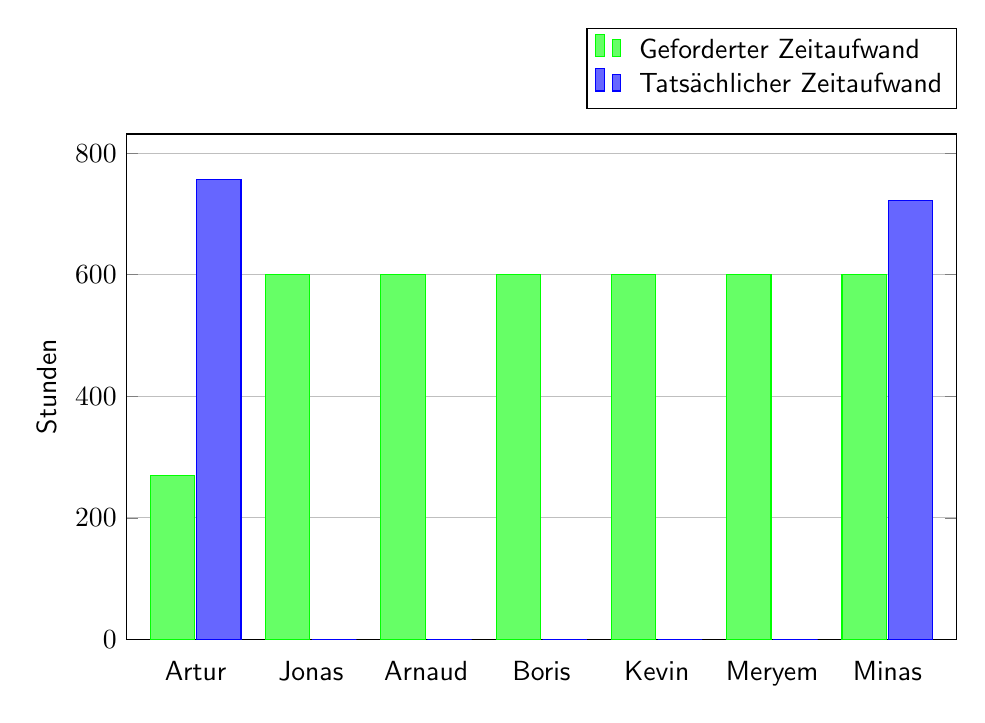
\begin{tikzpicture}
    \begin{axis}[
        width  = \textwidth,
        height = 8cm,
        major x tick style = transparent,
        ybar=2*\pgflinewidth,
        bar width=16pt,
        ymajorgrids = true,
        ylabel = {Stunden},
        symbolic x coords={Artur,Jonas,Arnaud,Boris,Kevin,Meryem,Minas},
        xtick = data,
        scaled y ticks = false,
        enlarge x limits=0.1,
        ymin=0,
        legend cell align=left,
        legend style={
                at={(1,1.05)},
                anchor=south east,
                column sep=1ex
        }
    ]
        \addplot[style={green,fill=green!60,mark=none}]
            coordinates {(Artur, 270) (Jonas,600) (Arnaud,600) (Boris,600) (Kevin,600) (Meryem,600) (Minas,600)};

        \addplot[style={blue,fill=blue!60,mark=none}]
             coordinates {(Artur,756) (Jonas,0) (Arnaud,0) (Boris,0) (Kevin,0) (Meryem,0) (Minas,722)};

        \legend{Geforderter Zeitaufwand,Tatsächlicher Zeitaufwand}
    \end{axis}
\end{tikzpicture} 
%\caption{Stundenaufwand: Vergleich zwischen gefoderten und tatsächlichen Zeitaufwand der Projektgruppenmitglieder.} 
\end{figure} 



\subsection{Verantwortungsbereiche}
Innerhalb der Projektgruppe (PG) war ein Ziel, dass jeder der Mitglieder "Experte" für einen Bereich wird. Damit haben wir die Verantwortung relativ gleichmäßig auf alle aufgeteilt. Dazu muss noch erwähnt werden, dass die Teammitglieder nicht nur ausschließlich die Aufgaben des jeweiligen Verantwortungsbereiches erlegibt habe. Es wurde sich vielmehr gegenseitig immer unterstützt und viel zusammengearbeitet. Die Verantwortungsbereiche haben sich mit der Zeit folgendermaßen aufgeteilt: \\

$ \bullet $ Artur Piet: Mustererkennung, 3D-Konstruktion und Sprecher der PG \\
$ \bullet $ Jonas Pöhler: Hardware, Webanbindung und Stellv. Sprecher der PG \\
$ \bullet $ Arnaud Eric Toham Waffo: Elektrodenauswahl \\
$ \bullet $ Boris Kamdem: Langeweile-Szenario und Fragebogen in VR \\
$ \bullet $ Kevin Orth: Komplette Hardware \\
$ \bullet $ Meryem Dural: Frustations-Szenario in VR \\
$ \bullet $ Minas Michail: Glücks-Szenario in VR \\


\subsection{Gruppentreffen}
Die wöchentliche Gruppentreffen finden immer Donnerstags ab 14:00 Uhr statt und beginnen in der Regel mit einer Update-Runde. Hierbei kommen alle Gruppenteilnehmer der Reihe nach dran und jeder erklärt kurz woran letzte Woche gearbeitet wurde, was die aktuellen Herausfoderungen und Probleme sind und was genau als nächstes geplant ist. Ziel ist es den Austausch und die Kommunikation unter den Teammitgliedern und den Projektleitern zu fördern, damit alle Teilnehmer auf dem selben Wissenstand sind, da einzelnen Aufgaben durchaus großen Einfluß auf Tätigkeiten von anderen Mitgliedern haben können. \\


% 4 Grundlagen
\newpage
\section{Grundlagen} \label{grundlagen-sec}
\todo[inline]{Verantwortlich: Arnaud}



% Unterkapitel
\subsection{Definition von Emotionen} \label{definition-emotionen}


\todo[inline]{Verantwortlich: Arnaud}


Der Begriff ``Emotion'' wird zwar weltweit  (in fast allen Sprachen) und von alle Menschen verwendet (die soziale oder intellektuelle Ebene spielt keine Rolle), ist aber relativ schwer zu definieren. 
Dieses Paradox wurde bereits im folgenden Zitat explizit erwähnt: 
``Everybody knows what an emotion is, until asked to give a definition.''\cite{fehr_russel_1984} von Fehr und Russell, zwei amerikanischer Emotionsforscher (Psychologe). 
Noch überraschender ist die Schwankung in der Definition dieses Begriffs ``Emotion'' im Laufe der Zeit: Allein die englischsprachige Experimentalpsychologie\cite{plamper12} liefert zwischen 1872 und 1980 mehr als 92 verschiedene Definitionen. 
Wir verstehen daher, dass es schwierig wäre, zu versuchen, diese Definition zu formulieren.  
Wie können wir also die Schwierigkeit, eine Definition für einen solchen gemeinsamen Begriff zu finden, erklären? 
Man sollte nicht vergessen werden, dass es sich um einen eher abstrakten Begriff handelt und daher ist die Emotion sehr subjektiv. 
Neben diesem abstrakten Aspekt ist auch anzumerken, dass sich der Begriff der Emotion auch auf viele Bereiche bezieht, die sich ebenso voneinander unterscheiden wie sie variieren: z.B. Literatur, Philosophie, Psychologie usw. 
Neben diesem multidisziplinären Charakter, der die Pluralität der Vorstellungen und Ansätze in jedem Definitionsversuch erklären könnte, ist es auch notwendig, die Variationen von Sprachen, Perioden und sogar Kulturen hinzuzufügen. \\


Es wird uns allein mit dieser Arbeit (und das ist auch nicht von uns erwartet) nicht möglich sein, alle Fragen im Zusammenhang mit der Definition des Begriffs ``Emotion'' zu betrachten, aber wir werden einige konkrete Beispiele vorstellen, um die Komplexität zu veranschaulichen, die sich aus der Suche nach einer Definition von Emotion ergeben kann.  
Die antiken Philosophen\cite{geslin13} waren die ersten, die sich mit Emotionen und ihren Einflüssen auf den Alltag beschäftigen haben. 
Tatsächlich nahmen Stoiker wie Zeno und Plato bereits 370 n. Chr. Emotionen als eine Krankheit der Seele wahr, die für sie ein Hindernis für denjenigen war, der denken wollte. 
Platon geht mit seiner Allegorie von der Höhle tiefer, indem er alles was emotional ist  mit alle vernünftig (verständlich) kontrastiert: das heiß Emotion und Vernunft gehen nicht zusammen. 
Descartes und Aristoteles vervollständigen Platons Beobachtungen, indem sie in die Analyse von Emotionen eine Dualität (positiv und negativ) der Perzeption einbringen. 
Aristoteles glaubt, dass alles, was das Leben auf positive Weise beeinflusst, durch positive Emotionen bedingt ist, und Descartes glaubt, dass Emotionen für unser Überleben unerlässlich sind und dass die Schwäche eines Menschen eng mit der Fähigkeit der Seele verbunden ist, seine Emotionen zu kontrollieren. 
Charles Darwin in seinem präsentierte weitere ebenso faszinierende neue Elemente über Emotionen, ohne den bisherigen Beobachtungen zu widersprechen\cite{darwin1872}. 
Er verallgemeinert die Emotionen für alle Kulturen und fand sogar ähnlichkeit mit Tiere. 
Der Darwin präsentiert  Emotionen  als Körpersignale (oder Reaktionen) auf äußere Handlungen(Externe Ereignisse), begleitet von spezifischen körperlichen Äußerungen wie: Gesichtsausdrücke, Gesten und oft Geräusche, die alle  spezifisch je nach Emotionen sind. \\


So können wir weiterhin andere berühmte wissenschaftliche Namen wie William James\cite{james1884}, Walter Cannon\cite{cannon32}, Stanley Scharter\cite{schachter59} usw. nennen, die zu unterschiedlichen Zeiten und an unterschiedlichen Orten das Thema untersucht haben, mit ebenso relevanten wie unterschiedlichen Schlussfolgerungen, aber die Beobachtung bleibt die gleiche, die Definition bleibt unbeständig.
Neben den Schwierigkeiten, die sich aus den oben genannten unterschiedlichen Wahrnehmungen ergeben, trägt die  tägliche missbräuchliche Verwendung bestimmter Begriffe wie Gefühl, Affekt, Stimmung, Gefühl (um nur einige zu nennen) als Synonym für Emotionen dazu bei  mehr Verwirrung in das Verständnis von Emotionen. Diese Begriffe beziehen sich zwar auf Gemütszustände, sind aber jedoch nicht Synonym von Emotion\cite{plamper12}.
Trotz des fehlenden Konsenses über die Frage der Definition dieses Begriffs gibt es jedoch Elemente, die in allen Definitionsversuchen wiederkehren, nämlich: 

\begin{itemize} \setlength\itemsep{-0.15cm}
  \item das Vorhandensein eines Auslösers;
  \item den psychischen Zustand des Subjekts;
  \item einen bestimmten Körperausdruck;
  \item eine physiologische Reaktion (Herzfrequenz, Atmung,Schwitzen ...);
  \item eine bestimmte Qualität, Intensität und Dauer.
\end{itemize}


Basierend auf den obigen Elementen können wir daher zu dem Schluss kommen, dass wir zwar nicht genau definieren können, was eine Emotion ist, können wir aber jedoch jede davon mit Bestimmte spezifisch  Element in Verbindung setzen: einen Stimulus (der der Auslöser der Emotion ist), eine physiologische und körperliche Reaktion. 
Die Existenz mehrerer verschiedener Emotionen lässt sich gerade wegen der Spezifität dieser Elemente vermuten. 
Im nächsten Teil werden wir versuchen, die verschiedenen Emotionen zu klassifizieren, mit einem besonderen Fokus auf diejenigen, die wir zu induzieren versuchen. \\


Wie bei der Definition von Emotionen gibt es keine einheitliche Klassifizierung von Emotionen. 
Und wie bei den versuchten Definitionen gab es im Laufe der Zeit mehrere vorgeschlagene Klassifikationen, die sich auch im Laufe der Zeit entwickelt haben. 
Diese Mehrheit von klassifikationen ist vermutlich eine Folge des Mangels an Konsens über die Definition selbst. 
Es gibt jedoch zwei Arten von Klassifikationen, die vor allem unterscheidet und durchgesetzt haben: eine dimensionale Klassifikation\cite{geslin13} und eine kategorische Klassifikation\cite{basic_emotions_theories}.




\subsubsection{Kategoriale Klassifikation} \label{kategoriale-klassifikation}

Angetrieben von Charles Darwin, (der auch der erste war, der grundlegende Emotionen identifizierte) diese Vorgehensweise ist die von Emotionsforscher  mit einer evolutionären Ansatz. 
Diese Klassifikation basiert auf der Existenz von eine Reihe von sogenannten Grundemotionen oder primäre Emotionen. 
Diese  Emotionen wäre in einer begrenzten Anzahl und ihre Entwicklung wurde stark von der Evolution  beeinflusst. 
Wie viele Dinge in Bezug auf die Emotionen in allgemein, variiert die Anzahl von Grundemotionen von einem Emotionsforscher zu einem anderen (siehe Tabelle \ref{vergleich-basisemotionen}).


\begin{table}[h] \centering
\begin{tabular}{| p{5cm} | p{11cm} |}
\hline
\textbf{Forscher} & \textbf{Basisemotionen} \\ \hline
Gray (1982) & Furcht, Freude, Ärger \\ \hline
Panksepp (1982) & Furcht, Erwartung, Ärger, Panik \\  \hline
Tomkins (1984) & Furcht, Freude, Ärger, Verzweiflung, Ekel, Überraschung, Interesse, Scham, Zufriedenheit \\  \hline
Plutchik (1980) & Furcht, Freude, Ärger, Traurigkeit, Ekel, Überraschung, Akzeptanz, Erwartung \\  \hline
Arnold (1960) & Furcht, Liebe, Ärger, Traurigkeit, Hass, Hoffnung, Begehren, Mut, Niedergeschlagenheit, Verzweiflung, Widerwille \\  \hline
Oatley \& Johnson-Laird (1987) & Furcht, Glück, Ärger, Traurigkeit, Ekel \\  \hline
Ekman (1982) & Furcht, Freude, Ärger, Traurigkeit, Ekel, Überraschung \\  \hline
Izard (1987) & Furcht, Freude, Ärger, Traurigkeit, Ekel, Überraschung, Interesse,Verachtung \\ \hline
\end{tabular} \caption[Vergleich einige Basisemotions-Theorien]{ Vergleich einige Basisemotions-Theorien\cite{basic_emotions_theories}. } \label{vergleich-basisemotionen}
\end{table}



Obwohl sie sich nicht über die Anzahl der Grundemotionen einig sind, sind sich die Forscher einig über die Existenz komplexerer Emotionen, die die Kombination mehrerer primärer Emotionen wären. 
Basierend auf diesem Ansatz wurden mehrere Theorien entwickelt, um Emotionen darzustellen, von denen eine der bekannte das Plutchik-Modell ist. 
Plutchiks Modell verwendet ein radförmiges Diagramm (siehe Abbildung \ref{plutchik}) und verschiedene Farben, um jede Emotion darzustellen. \\


\begin{figure}[h]
\includegraphics[width=\textwidth]{Images/plutchik.png} 
\vspace{-0.3cm} 
\caption{ Einordnung von Emotion nach Plutchik. }
\label{plutchik} 
\end{figure}


Diese Theorie fundiert sich auf  das acht primäre Emotionen mit einer klare trennung (bzw unterschied) zwischen  primären, sekundären und tertiären Emotionen.
Die verbindet jede primäre Emotion mit spezifischen Motivationssystem und Verhaltendstedenze zur Bewältigung grundlegender adaptiver Probleme (siehe Tabelle \ref{verhalten-funktion}). 


\begin{table}[h] \centering
\begin{tabular}{| p{5.1cm} | p{5.1cm} | p{5.1cm} |}
\hline
\textbf{Subjektiv} & \textbf{Verhalten} & \textbf{Funktion} \\ \hline
Angst, Entsetzen & Rückzug, Flucht  & Schutz \\ \hline
Ärger, Wut & Angriff, Beißen & Zerstörung \\ \hline
Freude, Ekstase & Paarung, Besitz & ergreifen Fortpflanzung \\ \hline
Traurigkeit, Trauer & Weinen, Bitte um Hilfe & Reintegration \\ \hline
Akzeptanz, Anbetung, Vertrauen & Paarbildung, Pflege & Zusammengehörigkeit, Bindung \\ \hline
Ekel, Abscheu & Sich übergeben & Ablehnung, Zurückweisung \\ \hline
Erwartung, Antizipation & Untersuchen & Exploration, Erkundung \\ \hline
Überraschung & Innehalten, Einfrieren & Orientierung \\ \hline
\end{tabular} \caption[ Einige Basisemotionen jeweils mit Verhalten und Funktio ]{ Einige Basisemotionen jeweils mit Verhalten und Funktion\cite{basic_emotions_theories}. } \label{verhalten-funktion}
\end{table}






\subsubsection{Kategoriale Ansatz} \label{kategoriale-ansatz}

Dieser von Wundt\cite{basic_emotions_theories} initiierte Ansatz geht von dem Gedanken aus, dass die emotionale Erfahrung in einem mehrdimensionalen Raum dargestellt werden kann. 
Dieser Zerlegung der emotionale Erfahrung  sollte es ermöglichen, eine genaue Analogie zwischen Emotion und Körperausdruck (Gesichtsausdrücke) herzustellen. 
Dieser Ansatz wurde  daher den Vorteil, dass sie die Tür zu einer möglichen Quantifizierung der emotionalen Erfahrung öffnet. 
Die Idee von Wundt (siehe Abbildung \ref{wundt})  war einer dreidimensionalen Zerlegung(Lust-Unlust, Spannung-Entspannung (Lösung), Beruhigung (Ruhe)-Erregung siehe) der emotionalen Erfahrung. 


\begin{figure}[h]
\includegraphics[width=\textwidth]{Images/wundt.png} 
\vspace{-0.3cm} 
\caption[Einordnung von emotionale Erfahrungsprozess nach Wundt.]{ Einordnung von emotionale Erfahrungsprozess nach Wundt\cite{basic_emotions_theories}. }
\label{wundt} 
\end{figure}


Die Frage nach der Anzahl der Dimensionen, die zur Darstellung der emotionalen Erfahrung notwendig sind, wird jedoch zu mehreren Theorien führen. 
Allerdings schlug Russell\cite{basic_emotions_theories} eine zweidimensionale Darstellung mit sechs primären Emotionen nach Ekam vor (siehe Tabelle \ref{vergleich-basisemotionen}). 
Emotionen werden also dank dieses Modells (siehe Abbildung \ref{russell}) eine horizontale Komponente haben: Valenz (Freude/Verdruss) und eine vertikale Komponente: Erregung (Aktivierung). 


\begin{figure}[h] \centering
\includegraphics[width=12cm]{Images/russell.png} 
\vspace{-0.3cm} 
\caption[Einordnung von emotional Erfahrung nach Russell.]{ Einordnung von emotional Erfahrung nach Russell\cite{basic_emotions_theories}. }
\label{russell} 
\end{figure}


Die Valenz unterscheidet positive Emotionen von negative Emotionen, und die Erregung informiert über körperliche Erregung, die man durch die Anzahl von physiologischen Reaktion feststellen kann. 
Jede Emotion lässt sich als Kombination dieser beiden Parameter darstellen was für eine mathematische auswertung sehr hilfreich sein könnte. 
Dieses Modell hat viel Erfolg gehabt, da er die Darstellung von eine Unendlichkeit von Emotionen erlaubt hat. 
Trotz der unterschiedlichen Anzahl von Dimensionen von verschiedenen Autoren vorgeschlagen, die beiden Dimensionen von Russell (Valenz und Erregung) sind Faktoren die in fast alle Modelle dieses Ansatzes auftreten.





% Unterkapitel
\subsection{Virtual Reality (VR)} \label{grund-vr}


\todo[inline]{Verantwortlich: Arnaud, Boris}

% Unterkapitel
\subsection{Sensoren und biophysiologische Signale zur Emotionserkennung} \label{grund-sensoren-subsec}

\todo[inline]{Verantwortlich: Arnaud, Kevin}

% Unterkapitel
\input{Part-0/4-Grundlagen/3-Sensoren/1-temperatur}

% Unterkapitel
\input{Part-0/4-Grundlagen/3-Sensoren/2-bvp}

% Unterkapitel
\input{Part-0/4-Grundlagen/3-Sensoren/3-spo2}

% Unterkapitel
\input{Part-0/4-Grundlagen/3-Sensoren/4-gsr}

% Unterkapitel
\input{Part-0/4-Grundlagen/3-Sensoren/5-eeg}

% Unterkapitel
\input{Part-0/4-Grundlagen/3-Sensoren/6-eog}

% Unterkapitel
\input{Part-0/4-Grundlagen/3-Sensoren/7-ad-wandler}

% Unterkapitel
\input{Part-0/4-Grundlagen/4-Kommunikation/1-kommunikation}




% Unterkapitel


% Unterkapitel
\input{Part-0/4-Grundlagen/5-Mustererkennung/1-grundlagen-mustererkennung}


% Unterkapitel 
\input{Part-0/4-Grundlagen/5-Mustererkennung/2-emotion-recognition-chain}





% 5 SOA Analyse
\newpage
\section{State-of-the-Art Analyse} \label{soa-sec}
\todo[inline]{Verantwortlich: Jonas}

Die Detektion von Emotionen kann auf unterschiedlichste Art erfolgen. In der Literatur wird neben der Verarbeitung von Biosignalen mittlerweile häufig auf eine Detektion durch Kameras oder durch die Analyse von Sprache gesetzt.(vgl. \cite{}) \\

Die Analyse mittels einer Kamera und der Aufnahme von Gesichtsmimik oder Augenbewegung war in der vorliegenden Arbeit nicht möglich, da die HTC Vive die der Proband während des Experimentes trägt, einen Großteil des Gesichtes und damit die Mimik wie auch die Augen verdeckt. Eine Interaktion mit dem Probanden mittels Sprache war ebenfalls nicht vorgesehen. Dementsprechend blieb nur die Möglichkeit der Detektion von Emotionen mittels Biosignalen. Hierbei wird in der Literatur vor allem die Atemfrequenz, die Hautleitfähigkeit, die elektrische Herzaktivität, die EEG Ableitung und die EOG Ableitung heran gezogen.(vgl. \cite{}) \\

Zur Klassifizierung der Emotionen werden in der Literatur unterschiedliche Techniken verwendet. In neuerer Zeit konzentriert sich die Forschung dabei auf Machine Learning gestützte Ansätze.(vgl. \cite{}) Dabei wird zwischen supervised und unsupervised Modellen unterschieden. Bei den unsupervised Modellen wird insbesondere Sequential Floating Forward Search und k-Nearest Neighbour (k-NN) benutzt. Hierbei handelt es sich um Techniken zur Selektion relevanter Features beziehungsweise zur Klassifizierung von Features durch Gruppenbildung.  Auf der Seite der supervised Modelle sticht vor allem die Nutzung der Support Vecotor Machine (SVM) hervor.(vgl. \cite{}) Hierbei wird wie bei allen supervised Modellen ein Datensatz mit Labels genutzt um das Modell auf die zugrunde liegende Datenmenge zu trainieren. 




% Part 1
\newpage
\part{Erster Prototype}
\addtocontents{toc}{\protect\mbox{}\protect\hrulefill\par}


% 1 Systementwurf
\section{Systementwurf und Konzept} \label{systementwurf-sec}
\todo[inline]{Verantwortlich: Kevin, Jonas}



% Unterkapitel 
\subsection{Anforderungen} \label{anfoderungen-1}

Auf Grundlage der Ziele des Forschungsprojektes ELISE und dem Sichten und Vergleichen von mehr als 30 wissenschaftlichen Veröffentlichungen der letzten 15 Jahre, ergeben sich bestimmte
Anforderungen für den Entwurf eines eigenen Emotionserkennungssystems. Einige wissenschaftliche Veröffentlichungen sind dabei nicht außer Acht zu lassen. Die Foscher von T.
Sharma, S. Bhardwaj und H. B. Maringanti haben in ihrer Veröffentlichung Emotion Estimation
using Physiological Signals versucht, mit Hilfe von GSR, Herzschlagrate,
BVP und der Temperatur Aufschluss über die Emotionen Zorn, Angst, Freude und Traurigkeit
durch Stimulation verschiedener Songs und Videos zu erhalten. Sie erforschten, in
welchen Fällen sich die Körperleitfähigkeit je nach emotionalem Ausdruck unterschiedlich
verhält. H. F. Garcia, A. A. Orozco und M. A. Alvarez versuchten in ihrer Arbeit Dynamic
physiological signal analysis based on Fisher kernels for emotion recognition durch unterschiedliche Klassifizierungsmodelle, die Signale von EEG, EOG, EMG (Elektromyografie),
GSR, Atmung und Temperatur zu analysieren. Dafür wurden 32 Probanden,
die ein 40-minütiges Video mit Musikausschnitten ansahen, aufgezeichnet und ausgewertet.
Durch ein automatisches Regressionsprozess-Modell verbesserten sie dynamische Merkmale
und weitere aufgezeichnete Signale für eine weiterführende Auswertung.
Die Emotionserkennung erfolgte bis vor einigen Jahren in Verbindung mit zusätzlichen Kameras
und Software zur Gesichtsmimik-Erkennung oder Stimmerkennung, nicht jedoch mit
einer reinen Aufnahme von Körpermesswerten. In ELISE sollen insbesondere die lernrelevanten Emotionen Langweile, Frustration, Verwirrung sowie Engagement und Freude erkannt
werden. Die Hardware-Architektur muss auch in diesem Fall wieder das Ziel erfüllen, dass
das Gefühl der Immersion nicht gestört wird. Das heißt, dass das System zur Erkennung von
lernrelevanten Emotionen an möglichst wenigen Stellen am Körper mit zusätzlicher Sensorik
angebracht wird.
Auf Basis der Literaturrecherche, wie in der Bibliographie ausgewiesen, sind folgende Sensoren
zur Aufnahme der lernrelevanten Emotionen ausgewählt worden:

• Gehirnaktivität (EEG)
• Augenbewegung (EOG)
• Blutvolumenpuls (BVP)
• Sauerstoffsättigung im Blut (PPG)
• Hautleitfähigkeit (GSR)
• Körpertemperatur

Da die Sensorwerte zum Mikrocontroller aufgrund ihres räumlichen Abstandes über den
Bus übertragen werden, unterliegen diese Werte den Zeitanforderungen des Datenbusses.
Hier ist zu überprüfen, welches Buskonzept den Zeitanforderungen gewachsen ist.
Um den Aufwand für den Benutzer gering zu halten und die Immersion nicht zu stören,
wird versucht, die Sensorik direkt an der VR-Brille anzubringen. Für die EEG- und
EOG-Sensoren ist dies sowieso notwendig, da diese Messungen lediglich am Kopf stattfinden
können. Zudem soll das Endsystem echtzeitfähig sein, um in der späteren Anwendung
Änderungen und Fluktuationen der Emotionen erkennen zu können und die Schulungen auf
den Lernenden anzupassen. Das Emotionserkennungssystem soll mobil anwendbar sein, da
neuere Versionen der HTC Vive VR-Brille in Zukunft den kabellosen Betrieb unterstützen.
Auch aus diesem Grund ist die Kompaktheit, Energieeffizienz und die Datenübertragung der
einzelnen Sensoren und die Datenübertragung des späteren Gesamtsystems, die ebenfalls
kabellos stattfinden soll, von großem Interesse. Eine mögliche Stelle zur Unterbringung des
Gesamtsystems wäre am Hinterkopf des Probanden, da dort der nötige Platz vorhanden ist
und erforderliche Befestigungsstellen am Kopfband der HTC Vive von Vorteil sind.



% Unterkapitel 
\subsection{Konzept} \label{konzept-1}

Auf Abbildung 1 kann man das Konzept der Architektur erkennen, Dies ist zur besseren Anschauung stark vereinfacht. Hierbei bildet der Mikrocontroller das zentrale Element, welches die einzelnen Sensoren anbindet, steuert und die Messsignale grob zur besseren Auswertung verarbeitet. Zur besseren und möglichst in Echtzeit stattfindeten Verarbeitung werden die Daten an einen externen Rechner weitergeleitet. In der Abbildung findet diese Weiterleitung Drahtlos mittels Bluetooth statt. Es wurden in den verschiedenen Prototypen für diese Zwecke sowohl Bluetooth als auch WLAN verwendet. Für die Teilsysteme EEG und EOG wurden schon einfache Physische Filter auf den Leiterplatten vorgesehen, welche die analogen Signale vorberarbeiten, bevor dies von einem AD-Wandler digitalisiert werden. Da die Elektroden für die EEG und EOG Messung nur am Kopf angebracht werden können, empfiehlt es sich die übrigen festgelegten Werte ebenfalls am Kopf zu messen. Um die Messung für möglichst viele Personen mit unterschiedlichen Kopfformen zu ermöglichen wurde zuerst ein elastisches Kopfband und später eine flexible Maske verwendet. All dies wurde für eine spätere Verwendung mit (unter) einer VR-Brille designet. 





% Unterkapitel
\subsection{Hardwareauswahl} \label{hardwareauswahl-1}



% Unterkapitel 
\input{Part-1/1-Systementwurf/3-Hardwareauswahl/1-auswahlkriterien}

% Unterkapitel 
\input{Part-1/1-Systementwurf/3-Hardwareauswahl/2-festlegung-hardware}



% Unterkapitel
\subsection{Hardwarearchitektur} \label{hardwarearchitektur-1}

In den nächsten Abschnitten werden die verwendeten Sensoren, sowie die dazugehörigen Messschaltungen näher erläutert. Im Rahmen dieser Projektgruppe wurden insgesamt drei Prototypen gefertigt. In einigen Fällen ist der Sensor, und die dazugehörige Schaltung  unverändert geblieben. Bei anderen Sensoren gab es Änderungen. In diesem Fall werden die Sensoren und Schaltungen für jeden Prototypen aufgeführt und erläutert.

Die Auswahl der zur Emotionsbestimmung nötigen Vitaldaten wurde im Rahmen der bereits erwähnten aufbauenden Masterarbeit von David Krönert bestimmt. Dies waren die Körpertemperatur, Sauerstoffsättigung im Blut, Blutvolumenpuls, Hautleitfähigkeit, Gehirnaktivität und die Augenbewegungen. Diese Auswahl von relevanten Vitaldaten wurde im leufe der Projektgruppe nicht mehr geändert. Einzig die genaue Art der Messung hat sich mit den unterschiedlichen Varianten des Messboards geändert. Im folgenden soll deshalb noch eine kurze Erklärung der einzelnen Sensoren erfolgen, und wie sich diese für unterschiedliche Prototypen geändert haben.  

% Unterkapitel
\input{Part-1/1-Systementwurf/4-Hardwarearchitektur/1-gsr}

% Unterkapitel
\input{Part-1/1-Systementwurf/4-Hardwarearchitektur/2-temperatur}

% Unterkapitel 
\input{Part-1/1-Systementwurf/4-Hardwarearchitektur/3-pulsoximeter}

% Unterkapitel 
\input{Part-1/1-Systementwurf/4-Hardwarearchitektur/4-eeg}

% Unterkapitel 
\input{Part-1/1-Systementwurf/4-Hardwarearchitektur/5-eog}

% Unterkapitel
\input{Part-1/1-Systementwurf/4-Hardwarearchitektur/6-datenuebertragung}



% Unterkapitel 
\subsection{Programmierung} \label{programmierung-1}







% Unterkapitel 
\subsection{Aufnahme der {\"u}bertragenen Daten} \label{aufnahme-daten-subsec}

Obwohl mit diesem Prototypen keine Messungen mit Emotionsinduktionen an Probanden durchgeführt wurden, fanden zu Testzwecken natürlich auch hier Datenaufnahmen statt. Diese Daten wurden auch wieder mit SerialPlot erfasst, da hier durch die visuelle Darstellung eine relativ schnelle Beurteilung der Daten möglich war. Anders als im Vorhergehenden Prototypen wurde allerdings nicht mehr auf die Bluetooth-Schnittelle zurückgegriffen. Hier wurden die Daten noch über die eingebaute USB-Schnittstelle übertragen, um mögliche Übertragungsfehler einer drahtlosen Verbindung auszuschließen. Das im ESP32 integrierte WLAN-Modul kam hier also noch nicht zum Einsatz.




% 2 Realisierung
\newpage
\section{Realisierung} \label{realisierung-sec}
\todo[inline]{Verantwortlich: Jonas, Kevin \\
- Next Step: Gliederung erstellen}




% 3 Emotionsinduktion
\newpage
\section{Emotionsinduktion} \label{emotionsinduktion-sec}
\todo[inline]{Verantwortlich: Minas}


Das Kapitel beinhaltet einen Ablauf, die verwendeten Fragebögen und die genutzten Szenarien (Glück, Langeweile, Frustration) der Emotionsinduktion für den ersten Prototypen. 
Kapitel Ablauf beschreibt in welcher Reihenfolge die Szenarien und die Fragebögen aufgerufen wurden. 
In den Kapiteln Fragebogen, Glücks- ,Langeweile- und Frustration-Szenario wird, die Entwicklung und Implementierung erläutert. 
Die Emotioninduktion des ersten Prototypen wurde nicht in einer VR-Umgebung entwickelt. 
Zudem muss angemerkt werden, dass diese Emotionsinduktion für eine Zwischenstudie diente. 
Dadurch wurde der Fokus nicht auf die Implementierung gelegt, welche verschiedene Formate besaß z.B. HTML oder PowerPoint, sondern auf den Inhalt, welches der Proband zu sehen oder zu hören bekam.
Die Emotionsinduktion wurde sowohl in Englisch als auch in Deutsch angeboten.



% Unterkapitel
\subsection{Ablauf} \label{ablauf-subsubsec}


\todo[inline]{Verantwortlich: Minas}


% Unterkapitel 
\subsection{Fragebogen} \label{fragebogen-4}


\todo[inline]{Verantwortlich: Boris}

F{\"u}r dieses Prototyp wurden zwei Arten von Frageb{\"o}gen benutzt. 
Der erste Typ ist sehr {\"a}hnlich mit dem von der zweite Prototyp. Es enth{\"a}lt in dem informativen Teil einen Text, wo es beschrieben wird, wie der Fragebogen ausgef{\"u}llt werden soll. Der andere Teil besteht aus vier Dropdown-Boxen von dreizehn Optionen, die zw{\"o}lf verschiedene Emotionen und einen als null oder neutral geltenden Zustand enthalten. Jede Dropdown-Box entspricht ein Viertelzeit der Szenario. Es soll zwischen die Optionen jeder Dropdown-Box gew{\"a}hlt werden, welche Emotion es am st{\"a}rksten empfindet wird, je nachdem, wann man es f{\"u}hlte, d.h. ob es das erste, zweite, dritte oder letzte Quartal der Zeit des Videos war, um die Emotion zu bew{\"a}ltigen. Unten gibt es ein Button wo man dr{\"u}cken kann, wenn man fertig ist. Allerdings hat man auch die M{\"o}glichkeit seine Wahl zu {\"a}ndern, auch wenn man sich schon im n{\"a}chsten Schritt befindet, indem man in diesem n{\"a}chsten Schritt auf den Zur{\"u}ck-Button dr{\"u}ckt und die gew{\"u}nschten {\"a}nderungen vornimmt. Hierf{\"u}r wird ein Widget Blueprint erstellt, die vier Dropdown-Boxen mit dem gew{\"u}nschten Anzahl an Optionen hinzugef{\"u}gt und die Labels von der unterschiedlichen Optionen der Dropdown-Boxen definiert. Ein Button ``next'' wird auch erstellt um zum n{\"a}chsten Fragebogen zu navigieren. Es wird auch eine zwischen Speicherungsfunktion in ein anderes Skript definiert, die hier aufgerufen wird, um die {\"a}nderung auch nach das dr{\"u}cken von dem ``next'' Button zu Speichern. Dabei wird vier Variablen definiert und die Werte von der gew{\"a}hlten Optionen werden ihnen zugewiesen. \\

(Bild f{\"u}r Fragebogen) \\


Der zweite Typ {\"a}hnelt dem ber{\"u}hmten Modell von James Russels ``circumplex'' \cite{russel_1980}. Es ist ein klassisches Modell mit einer kreisf{\"o}rmigen Struktur, die auf zwei senkrechten Diagonalen ruht. Die vertikale Achse, die die Erregung darstellt, und die horizontale Achse, die die Valenz darstellt. Das Zentrum des Kreises stellt eine neutrale Valenz und ein mittleres Erregungsniveau dar. Andere Emotionen werden auf jeder Ebene des Kreises dargestellt.  Hier wird ein weniger bekanntes Modell verwendet, das ``Self Assessment Manikin'' (SAM). Es besteht aus drei Reihen mit je f{\"u}nf Piktogrammen. Diese Piktogramme stellen den Zustand eines Gesichts nach verschiedenen Arten von Emotionen dar. So repr{\"a}sentiert der erste Bereich die Wertigkeit, der zweite die Erregung und der dritte die Dominanz. Eine Erkl{\"a}rung zu jedem dieser Begriffe ist ebenfalls neben dem Fragebogen enthalten, um die Testpersonen {\"u}ber diese W{\"o}rter aufzukl{\"a}ren.  Bei jeder Avatar und in der Mitte jeder der beiden Avatar befindet sich ein Checkbox.  So muss man f{\"u}r jede Zeile das Checkbox ausw{\"a}hlen, das ihrem emotionalen Zustand am besten entspricht. Man kann nur ein Checkbox pro Zeile markieren und man hat auch die M{\"o}glichkeit wie bei dem ersten Model seine Wahl zu {\"a}ndern. Es kann einfach mit Branch-Bedingungen realisieren werden.  Diese werden auch in eine Widget Blueprint wie f{\"u}r das erste Modell gemacht. Es gibt auch wieder die zwischen Speicherungsfunktion und das Button ``next''. Was neues hier kommt ist das Button ``back'' um wieder zum ersten Fragebogen zu navigieren. 

(Bild f{\"u}r circumplex) \\

% Unterkapitel 
\subsection{Szenarien} \label{szenarien-1}

\todo[inline]{Verantwortlich: Meryem}


Im Folgenden Kapitel werden drei verschiedene Szenarien dargeboten. Die Emotionen Glück, Langweile und Frustration werden hierfür zunächst erläutert. Für jede dieser Emotionen werden Szenarien vorgestellt, bei welchen diese bei den Probanden ausgelöst bzw angeregt werden sollen.


% Unterkapitel 
\input{Part-1/3-Emotionsinduktion/3-Szenarien/1-glueck}

% Unterkapitel 
\input{Part-1/3-Emotionsinduktion/3-Szenarien/2-langeweile}

% Unterkapitel 
\input{Part-1/3-Emotionsinduktion/3-Szenarien/3-frust}


% 4 Messreihe
\newpage


Die zweite Messreihe fand in zwei Räumen des Forschungskolleg Siegens (FoKoS) statt. Die Messreihe wurde in den beiden Wochen vom  14.01.19 bis 25.01.19 statt. Insgesamt wurden Daten von Daten von 97 Personen erhalten. Diese deutliche Steigerung der Teilnehmerzahl im Vergleich zur ersten Messreihe (hier waren es 22 Teilnehmer) wurde durch eine Auszahlung von 10€ erreicht. Bei der vorherigen Messreihe wurde an die Teilnehmer keine Aufwandsentschädigung für die Teilnahme geleistet. Eine genaue Auswertung der Daten folgt in späteren Kapiteln. Von der reinen Durchführung her lässt sich aber sagen, dass es mit nur einer Ausnahme keine Probleme bezüglich VR gab (Schwindel). Die Messungen wurden mit der an vorheriger Stelle schon beschriebenem dritten Prototypen gemacht Abb.1 . Das Messsystem bestand aus dem dritten Prototypen, der in einem extra hierfür gefertigten Gehäuse verbaut wurde. Zusätzlich wurde die in Realisierung beschriebene Maske verwendet. 


% 5 Mustererkennung
\newpage
\section{Mustererkennung} \label{mustererkennung-sec}

\todo[inline]{Verantwortlich: Artur\\
- RfP}

Da an dem ersten Tag der Messreihe noch Probleme bei der Datenversendung bestanden, wurden von den insgesamt 97 getesteten Probenden nur die Daten von nur 88 Personen analysiert.
Mit dem relativ großen Datensatz von 88 Testpersonen, wurde sich entschieden die Mustererkennung vor allem auf DNN-Ansätze mit Verwendung von den Circumplex-Labels zu fokusieren.
Die Gründe dafür waren, dass sich durch dieses Vorgehen die besten Ergebnisse erhofft wurden und ein gewisser Zeitdruck durch das anstehende Projektende.
Die getesteten DNN-Ansätze wurden bereits ausführlich in Kapitel \ref{dnn-1} erklärt.
Weitere Informationen zu den verwendeten Circumplex-Lables können in Kapitel \ref{fragebogen-4} nachgeschlagen werden.

% 6 Ergebnisse
\newpage
\section{Ergebnisse} \label{ergenisse-sec}
\todo[inline]{Verantwortlich: Artur}



% Unterkapitel 
\subsection{Ergebnisse der hand-gefertigten Merkmale} \label{ergebnisse-hc-features-subsec}

Von den insgesamt 22 Probenden wurden bei 7 Elektrodenproblemen festgestellt, weshalb die Qualität der Sensordaten bei diesen 7 Testpersonen angezweifelt wird.
Aus diesem Grund, wurden diese Daten für die Mustererkennung nicht berücksichtigt und der tatsächlich analysierte Datensatz besteht aus insgesamt 15 Probanden.
Zun{\"a}chst wurden die Daten mit einer Normalisierungstechnik vorverarbeitet, die bereits im Kapitel \ref{datenerfassung-0} beschrieben wurde.
Entsprechend der ERC wurde dann den gleitenden Zeitfenster-Segmentierungsansatz (vgl. Kapitel \ref{segmenation-1}) mit den Parametern $T=120$ und $\sigma=30$ verwendet.
Um die optimalen Parameter des SVM-Klassifikators (d.h. Soft-Margin $C$ und Kernelparameter $\gamma$) zu bestimmen, wurde ein Gitter-Suchansatz verwendet.
Es besteht darin, einen Satz m{\"o}glicher Werte f{\"u}r jeden Parameter zu definieren und die Leistungen des Klassifikators f{\"u}r jedes Paar m{\"o}glicher Werte zu testen (d.h. an jedem ``Knoten des Gitters''). \\

\begin{figure}[h]\centering{ \hspace{1cm}
\includegraphics[width=6cm]{Images/grid.png}}
\vspace{0.2cm} \caption[Gitter-Suche]{ Gitter-Suche: Ein definierter Satz m{\"o}glicher Werte f{\"u}r jeden Parameter wird an jedem ``Knoten des Gitters'' getestet. Diese Knoten sind in der Abbildung als rote Punkte markiert. }
\end{figure} 
\vspace{0.5cm}

Die folgenden Werte f{\"u}r $\gamma$ und $C$ wurden getestet:
\begin{center}
${\displaystyle \gamma \in \{0.002; 0.008; 0.03; 0.15; 0.5; 1; 2\}}$ \\
${\displaystyle C \in \{ 0.5; 1; 2; 8; 32; 128; 512 \}}$ \\
\end{center}
\vspace{0.5cm}

Da alle Probanden nicht alle Ziel-Emotionen erlebt bzw. angegeben haben, konnte die Leave-One-Subject-Out Kreuzvalidierung nur bedingt f{\"u}r die Bewertung angewendet werden.
Wir haben daher eine 5-fache Kreuzvalidierung mit entsprechendem F1-Wert verwendet. 

\begin{table}[h]
\center{
\begin{tabular}{|c|c|c|c|c|c|}
\hline
 \textbf{Fold 1} & \textbf{Fold 2} & \textbf{Fold 3} & \textbf{Fold 4} & \textbf{Fold 5} & \textbf{Durchschnitt} \\ \hline
 90.18 & 93.06 & 91.63 & 90.61 & 91.98 & 91.49 \\ \hline
\end{tabular}} \vspace{0.3cm} \caption[Durchschnittlicher F1-Wert]{ Durchschnittlicher F1-Wert in \% f{\"u}r die f{\"u}nf Falten des Datensatzes. }
\end{table}
\vspace{0.5cm}



Die Ergebnisse unserer Experimente zeigen, dass ein solcher Aufbau die Erzielung einer relativ hohen Genauigkeit f{\"u}r die Erkennung der vier Klassen erm{\"o}glicht.
Die Confusion-Matrizen f{\"u}r den handgefertigten Merkmalsansatz unter Verwendung der SVM-Klassifikation ist in der folgenden Tabelle zu finden.

\begin{table}[h]
\center{
\begin{tabular}{|c|c|c|c|c|}
\hline
  & \textbf{Sonstige} & \textbf{Gl{\"u}ck} & \textbf{Frustation} & \textbf{Langeweile} \\ \hline
 \textbf{Sonstige} & \textbf{95.21} & 1.98 & 0.29 & 2.51 \\ \hline
 \textbf{Gl{\"u}ck} & 7.84 & \textbf{90.93} & 0.39 & 0.84 \\ \hline
 \textbf{Frustation} & 8.49 & 2.50 & \textbf{84.14} & 4.87 \\ \hline
 \textbf{Langeweile} & 5.69 & 0.70 & 0.94 & \textbf{92.67} \\ \hline
\end{tabular}} \vspace{0.3cm} \caption[Confusion Matrix]{ Confusion Matrix in \% f{\"u}r die f{\"u}nf Falten des Datensatzes. }
\end{table}


% Unterkapitel 
\subsubsection{Codebook Approach} \label{codebook-approach-subsubsec}







% Unterkapitel
\subsection{Analyse der Ergebnisse} \label{analyse-subsec}


Es sei darauf hingewiesen, dass Lösungen, die auf der Verwendung von Deep Neural Networks (DNNs) zur Extraktion von Merkmalen basieren (z.B. Multi-Layer-Perceptron, Convolutional Neural oder Long-Short-Term-Memory Networks) ebenfalls getestet wurden. Diese Ansätze konnten aber nicht so gute Ergebnisse erzielen, wie die handgefertigten Merkmale. Erkennungsraten für die am wenigsten vertretenen Klassen (insbesondere ``Frustration'') scheinen der Grund für die schwache Performance der DNNs zu sein. Wir gehen davon aus, dass dieses Phänomen durch die relativ geringe Größe unseres Datensatzes verursacht wird. \\

Die schächere Performance des CA hat uns auch überrascht. Der Grund hierfür ist aber sehr wahrscheinlich der selbe wie bei den  DNNs, und zwar der relativ kleine Datensatz. \\

Allgemein deuten die Ergebnisse aber darauf hin, dass unser biomedizinisches Datenerfassungssystem zur Emotionserkennung erfolgreich eingesetzt werden könnte, um ein intelligent adaptives Lernsystems zu verbessern. Zukünftige Arbeiten werden die Verfeinerung des Multisensor-Datenerfassungsgerätes, die Erfassung weiterer und größerer Datensätze für die weitere Mustererkennungsanalyse und die Analyse der Wirksamkeit des Emotionserkennungssystems in einem VR-affektiven Lernkontext beinhalten.




% Part 2
\newpage
\part{Zweiter Prototype}
\addtocontents{toc}{\protect\mbox{}\protect\hrulefill\par}


% 1 Systementwurf
\section{Systementwurf und Konzept} \label{systementwurf-2}
\todo[inline]{Verantwortlich: Kevin, Jonas}



% Unterkapitel 
\subsection{Anforderungen} \label{anfoderungen-1}

Auf Grundlage der Ziele des Forschungsprojektes ELISE und dem Sichten und Vergleichen von mehr als 30 wissenschaftlichen Veröffentlichungen der letzten 15 Jahre, ergeben sich bestimmte
Anforderungen für den Entwurf eines eigenen Emotionserkennungssystems. Einige wissenschaftliche Veröffentlichungen sind dabei nicht außer Acht zu lassen. Die Foscher von T.
Sharma, S. Bhardwaj und H. B. Maringanti haben in ihrer Veröffentlichung Emotion Estimation
using Physiological Signals versucht, mit Hilfe von GSR, Herzschlagrate,
BVP und der Temperatur Aufschluss über die Emotionen Zorn, Angst, Freude und Traurigkeit
durch Stimulation verschiedener Songs und Videos zu erhalten. Sie erforschten, in
welchen Fällen sich die Körperleitfähigkeit je nach emotionalem Ausdruck unterschiedlich
verhält. H. F. Garcia, A. A. Orozco und M. A. Alvarez versuchten in ihrer Arbeit Dynamic
physiological signal analysis based on Fisher kernels for emotion recognition durch unterschiedliche Klassifizierungsmodelle, die Signale von EEG, EOG, EMG (Elektromyografie),
GSR, Atmung und Temperatur zu analysieren. Dafür wurden 32 Probanden,
die ein 40-minütiges Video mit Musikausschnitten ansahen, aufgezeichnet und ausgewertet.
Durch ein automatisches Regressionsprozess-Modell verbesserten sie dynamische Merkmale
und weitere aufgezeichnete Signale für eine weiterführende Auswertung.
Die Emotionserkennung erfolgte bis vor einigen Jahren in Verbindung mit zusätzlichen Kameras
und Software zur Gesichtsmimik-Erkennung oder Stimmerkennung, nicht jedoch mit
einer reinen Aufnahme von Körpermesswerten. In ELISE sollen insbesondere die lernrelevanten Emotionen Langweile, Frustration, Verwirrung sowie Engagement und Freude erkannt
werden. Die Hardware-Architektur muss auch in diesem Fall wieder das Ziel erfüllen, dass
das Gefühl der Immersion nicht gestört wird. Das heißt, dass das System zur Erkennung von
lernrelevanten Emotionen an möglichst wenigen Stellen am Körper mit zusätzlicher Sensorik
angebracht wird.
Auf Basis der Literaturrecherche, wie in der Bibliographie ausgewiesen, sind folgende Sensoren
zur Aufnahme der lernrelevanten Emotionen ausgewählt worden:

• Gehirnaktivität (EEG)
• Augenbewegung (EOG)
• Blutvolumenpuls (BVP)
• Sauerstoffsättigung im Blut (PPG)
• Hautleitfähigkeit (GSR)
• Körpertemperatur

Da die Sensorwerte zum Mikrocontroller aufgrund ihres räumlichen Abstandes über den
Bus übertragen werden, unterliegen diese Werte den Zeitanforderungen des Datenbusses.
Hier ist zu überprüfen, welches Buskonzept den Zeitanforderungen gewachsen ist.
Um den Aufwand für den Benutzer gering zu halten und die Immersion nicht zu stören,
wird versucht, die Sensorik direkt an der VR-Brille anzubringen. Für die EEG- und
EOG-Sensoren ist dies sowieso notwendig, da diese Messungen lediglich am Kopf stattfinden
können. Zudem soll das Endsystem echtzeitfähig sein, um in der späteren Anwendung
Änderungen und Fluktuationen der Emotionen erkennen zu können und die Schulungen auf
den Lernenden anzupassen. Das Emotionserkennungssystem soll mobil anwendbar sein, da
neuere Versionen der HTC Vive VR-Brille in Zukunft den kabellosen Betrieb unterstützen.
Auch aus diesem Grund ist die Kompaktheit, Energieeffizienz und die Datenübertragung der
einzelnen Sensoren und die Datenübertragung des späteren Gesamtsystems, die ebenfalls
kabellos stattfinden soll, von großem Interesse. Eine mögliche Stelle zur Unterbringung des
Gesamtsystems wäre am Hinterkopf des Probanden, da dort der nötige Platz vorhanden ist
und erforderliche Befestigungsstellen am Kopfband der HTC Vive von Vorteil sind.



% Unterkapitel 
\subsection{Konzept} \label{konzept-1}

Auf Abbildung 1 kann man das Konzept der Architektur erkennen, Dies ist zur besseren Anschauung stark vereinfacht. Hierbei bildet der Mikrocontroller das zentrale Element, welches die einzelnen Sensoren anbindet, steuert und die Messsignale grob zur besseren Auswertung verarbeitet. Zur besseren und möglichst in Echtzeit stattfindeten Verarbeitung werden die Daten an einen externen Rechner weitergeleitet. In der Abbildung findet diese Weiterleitung Drahtlos mittels Bluetooth statt. Es wurden in den verschiedenen Prototypen für diese Zwecke sowohl Bluetooth als auch WLAN verwendet. Für die Teilsysteme EEG und EOG wurden schon einfache Physische Filter auf den Leiterplatten vorgesehen, welche die analogen Signale vorberarbeiten, bevor dies von einem AD-Wandler digitalisiert werden. Da die Elektroden für die EEG und EOG Messung nur am Kopf angebracht werden können, empfiehlt es sich die übrigen festgelegten Werte ebenfalls am Kopf zu messen. Um die Messung für möglichst viele Personen mit unterschiedlichen Kopfformen zu ermöglichen wurde zuerst ein elastisches Kopfband und später eine flexible Maske verwendet. All dies wurde für eine spätere Verwendung mit (unter) einer VR-Brille designet. 





% Unterkapitel
\subsection{Hardwareauswahl} \label{hardwareauswahl-1}



% Unterkapitel 
\input{Part-1/1-Systementwurf/3-Hardwareauswahl/1-auswahlkriterien}

% Unterkapitel 
\input{Part-1/1-Systementwurf/3-Hardwareauswahl/2-festlegung-hardware}



% Unterkapitel
\subsection{Hardwarearchitektur} \label{hardwarearchitektur-1}

In den nächsten Abschnitten werden die verwendeten Sensoren, sowie die dazugehörigen Messschaltungen näher erläutert. Im Rahmen dieser Projektgruppe wurden insgesamt drei Prototypen gefertigt. In einigen Fällen ist der Sensor, und die dazugehörige Schaltung  unverändert geblieben. Bei anderen Sensoren gab es Änderungen. In diesem Fall werden die Sensoren und Schaltungen für jeden Prototypen aufgeführt und erläutert.

Die Auswahl der zur Emotionsbestimmung nötigen Vitaldaten wurde im Rahmen der bereits erwähnten aufbauenden Masterarbeit von David Krönert bestimmt. Dies waren die Körpertemperatur, Sauerstoffsättigung im Blut, Blutvolumenpuls, Hautleitfähigkeit, Gehirnaktivität und die Augenbewegungen. Diese Auswahl von relevanten Vitaldaten wurde im leufe der Projektgruppe nicht mehr geändert. Einzig die genaue Art der Messung hat sich mit den unterschiedlichen Varianten des Messboards geändert. Im folgenden soll deshalb noch eine kurze Erklärung der einzelnen Sensoren erfolgen, und wie sich diese für unterschiedliche Prototypen geändert haben.  

% Unterkapitel
\input{Part-1/1-Systementwurf/4-Hardwarearchitektur/1-gsr}

% Unterkapitel
\input{Part-1/1-Systementwurf/4-Hardwarearchitektur/2-temperatur}

% Unterkapitel 
\input{Part-1/1-Systementwurf/4-Hardwarearchitektur/3-pulsoximeter}

% Unterkapitel 
\input{Part-1/1-Systementwurf/4-Hardwarearchitektur/4-eeg}

% Unterkapitel 
\input{Part-1/1-Systementwurf/4-Hardwarearchitektur/5-eog}

% Unterkapitel
\input{Part-1/1-Systementwurf/4-Hardwarearchitektur/6-datenuebertragung}



% Unterkapitel 
\subsection{Programmierung} \label{programmierung-1}







% Unterkapitel 
\subsection{Aufnahme der {\"u}bertragenen Daten} \label{aufnahme-daten-subsec}

Obwohl mit diesem Prototypen keine Messungen mit Emotionsinduktionen an Probanden durchgeführt wurden, fanden zu Testzwecken natürlich auch hier Datenaufnahmen statt. Diese Daten wurden auch wieder mit SerialPlot erfasst, da hier durch die visuelle Darstellung eine relativ schnelle Beurteilung der Daten möglich war. Anders als im Vorhergehenden Prototypen wurde allerdings nicht mehr auf die Bluetooth-Schnittelle zurückgegriffen. Hier wurden die Daten noch über die eingebaute USB-Schnittstelle übertragen, um mögliche Übertragungsfehler einer drahtlosen Verbindung auszuschließen. Das im ESP32 integrierte WLAN-Modul kam hier also noch nicht zum Einsatz.




% 2 Realisierung
\newpage
\section{Realisierung} \label{realisierung-2}
\todo[inline]{Verantwortlich: Jonas, Kevin \\
- Next Step: Gliederung erstellen}




\iffalse %comment everything till fi
% 3 Emotionsinduktion
\newpage
\section{Emotionsinduktion} \label{emotionsinduktion-2}
\todo[inline]{Verantwortlich: Minas}


Das Kapitel beinhaltet einen Ablauf, die verwendeten Fragebögen und die genutzten Szenarien (Glück, Langeweile, Frustration) der Emotionsinduktion für den ersten Prototypen. 
Kapitel Ablauf beschreibt in welcher Reihenfolge die Szenarien und die Fragebögen aufgerufen wurden. 
In den Kapiteln Fragebogen, Glücks- ,Langeweile- und Frustration-Szenario wird, die Entwicklung und Implementierung erläutert. 
Die Emotioninduktion des ersten Prototypen wurde nicht in einer VR-Umgebung entwickelt. 
Zudem muss angemerkt werden, dass diese Emotionsinduktion für eine Zwischenstudie diente. 
Dadurch wurde der Fokus nicht auf die Implementierung gelegt, welche verschiedene Formate besaß z.B. HTML oder PowerPoint, sondern auf den Inhalt, welches der Proband zu sehen oder zu hören bekam.
Die Emotionsinduktion wurde sowohl in Englisch als auch in Deutsch angeboten.



% Unterkapitel
\subsection{Ablauf} \label{ablauf-subsubsec}


\todo[inline]{Verantwortlich: Minas}


% Unterkapitel 
\subsection{Fragebogen} \label{fragebogen-4}


\todo[inline]{Verantwortlich: Boris}

F{\"u}r dieses Prototyp wurden zwei Arten von Frageb{\"o}gen benutzt. 
Der erste Typ ist sehr {\"a}hnlich mit dem von der zweite Prototyp. Es enth{\"a}lt in dem informativen Teil einen Text, wo es beschrieben wird, wie der Fragebogen ausgef{\"u}llt werden soll. Der andere Teil besteht aus vier Dropdown-Boxen von dreizehn Optionen, die zw{\"o}lf verschiedene Emotionen und einen als null oder neutral geltenden Zustand enthalten. Jede Dropdown-Box entspricht ein Viertelzeit der Szenario. Es soll zwischen die Optionen jeder Dropdown-Box gew{\"a}hlt werden, welche Emotion es am st{\"a}rksten empfindet wird, je nachdem, wann man es f{\"u}hlte, d.h. ob es das erste, zweite, dritte oder letzte Quartal der Zeit des Videos war, um die Emotion zu bew{\"a}ltigen. Unten gibt es ein Button wo man dr{\"u}cken kann, wenn man fertig ist. Allerdings hat man auch die M{\"o}glichkeit seine Wahl zu {\"a}ndern, auch wenn man sich schon im n{\"a}chsten Schritt befindet, indem man in diesem n{\"a}chsten Schritt auf den Zur{\"u}ck-Button dr{\"u}ckt und die gew{\"u}nschten {\"a}nderungen vornimmt. Hierf{\"u}r wird ein Widget Blueprint erstellt, die vier Dropdown-Boxen mit dem gew{\"u}nschten Anzahl an Optionen hinzugef{\"u}gt und die Labels von der unterschiedlichen Optionen der Dropdown-Boxen definiert. Ein Button ``next'' wird auch erstellt um zum n{\"a}chsten Fragebogen zu navigieren. Es wird auch eine zwischen Speicherungsfunktion in ein anderes Skript definiert, die hier aufgerufen wird, um die {\"a}nderung auch nach das dr{\"u}cken von dem ``next'' Button zu Speichern. Dabei wird vier Variablen definiert und die Werte von der gew{\"a}hlten Optionen werden ihnen zugewiesen. \\

(Bild f{\"u}r Fragebogen) \\


Der zweite Typ {\"a}hnelt dem ber{\"u}hmten Modell von James Russels ``circumplex'' \cite{russel_1980}. Es ist ein klassisches Modell mit einer kreisf{\"o}rmigen Struktur, die auf zwei senkrechten Diagonalen ruht. Die vertikale Achse, die die Erregung darstellt, und die horizontale Achse, die die Valenz darstellt. Das Zentrum des Kreises stellt eine neutrale Valenz und ein mittleres Erregungsniveau dar. Andere Emotionen werden auf jeder Ebene des Kreises dargestellt.  Hier wird ein weniger bekanntes Modell verwendet, das ``Self Assessment Manikin'' (SAM). Es besteht aus drei Reihen mit je f{\"u}nf Piktogrammen. Diese Piktogramme stellen den Zustand eines Gesichts nach verschiedenen Arten von Emotionen dar. So repr{\"a}sentiert der erste Bereich die Wertigkeit, der zweite die Erregung und der dritte die Dominanz. Eine Erkl{\"a}rung zu jedem dieser Begriffe ist ebenfalls neben dem Fragebogen enthalten, um die Testpersonen {\"u}ber diese W{\"o}rter aufzukl{\"a}ren.  Bei jeder Avatar und in der Mitte jeder der beiden Avatar befindet sich ein Checkbox.  So muss man f{\"u}r jede Zeile das Checkbox ausw{\"a}hlen, das ihrem emotionalen Zustand am besten entspricht. Man kann nur ein Checkbox pro Zeile markieren und man hat auch die M{\"o}glichkeit wie bei dem ersten Model seine Wahl zu {\"a}ndern. Es kann einfach mit Branch-Bedingungen realisieren werden.  Diese werden auch in eine Widget Blueprint wie f{\"u}r das erste Modell gemacht. Es gibt auch wieder die zwischen Speicherungsfunktion und das Button ``next''. Was neues hier kommt ist das Button ``back'' um wieder zum ersten Fragebogen zu navigieren. 

(Bild f{\"u}r circumplex) \\

% Unterkapitel 
\subsection{Szenarien} \label{szenarien-1}

\todo[inline]{Verantwortlich: Meryem}


Im Folgenden Kapitel werden drei verschiedene Szenarien dargeboten. Die Emotionen Glück, Langweile und Frustration werden hierfür zunächst erläutert. Für jede dieser Emotionen werden Szenarien vorgestellt, bei welchen diese bei den Probanden ausgelöst bzw angeregt werden sollen.


% Unterkapitel 
\input{Part-1/3-Emotionsinduktion/3-Szenarien/1-glueck}

% Unterkapitel 
\input{Part-1/3-Emotionsinduktion/3-Szenarien/2-langeweile}

% Unterkapitel 
\input{Part-1/3-Emotionsinduktion/3-Szenarien/3-frust}


% 4 Messreihe
\newpage
\section{Messreihe} \label{messreihe-2}


Die zweite Messreihe fand in zwei Räumen des Forschungskolleg Siegens (FoKoS) statt. Die Messreihe wurde in den beiden Wochen vom  14.01.19 bis 25.01.19 statt. Insgesamt wurden Daten von Daten von 97 Personen erhalten. Diese deutliche Steigerung der Teilnehmerzahl im Vergleich zur ersten Messreihe (hier waren es 22 Teilnehmer) wurde durch eine Auszahlung von 10€ erreicht. Bei der vorherigen Messreihe wurde an die Teilnehmer keine Aufwandsentschädigung für die Teilnahme geleistet. Eine genaue Auswertung der Daten folgt in späteren Kapiteln. Von der reinen Durchführung her lässt sich aber sagen, dass es mit nur einer Ausnahme keine Probleme bezüglich VR gab (Schwindel). Die Messungen wurden mit der an vorheriger Stelle schon beschriebenem dritten Prototypen gemacht Abb.1 . Das Messsystem bestand aus dem dritten Prototypen, der in einem extra hierfür gefertigten Gehäuse verbaut wurde. Zusätzlich wurde die in Realisierung beschriebene Maske verwendet. 


% 5 Mustererkennung
\newpage
\section{Mustererkennung} \label{mustererkennung-2}

\todo[inline]{Verantwortlich: Artur\\
- RfP}

Da an dem ersten Tag der Messreihe noch Probleme bei der Datenversendung bestanden, wurden von den insgesamt 97 getesteten Probenden nur die Daten von nur 88 Personen analysiert.
Mit dem relativ großen Datensatz von 88 Testpersonen, wurde sich entschieden die Mustererkennung vor allem auf DNN-Ansätze mit Verwendung von den Circumplex-Labels zu fokusieren.
Die Gründe dafür waren, dass sich durch dieses Vorgehen die besten Ergebnisse erhofft wurden und ein gewisser Zeitdruck durch das anstehende Projektende.
Die getesteten DNN-Ansätze wurden bereits ausführlich in Kapitel \ref{dnn-1} erklärt.
Weitere Informationen zu den verwendeten Circumplex-Lables können in Kapitel \ref{fragebogen-4} nachgeschlagen werden.

% 6 Ergebnisse
\newpage
\section{Ergebnisse} \label{ergenisse-2}
\todo[inline]{Verantwortlich: Artur}



% Unterkapitel 
\subsection{Ergebnisse der hand-gefertigten Merkmale} \label{ergebnisse-hc-features-subsec}

Von den insgesamt 22 Probenden wurden bei 7 Elektrodenproblemen festgestellt, weshalb die Qualität der Sensordaten bei diesen 7 Testpersonen angezweifelt wird.
Aus diesem Grund, wurden diese Daten für die Mustererkennung nicht berücksichtigt und der tatsächlich analysierte Datensatz besteht aus insgesamt 15 Probanden.
Zun{\"a}chst wurden die Daten mit einer Normalisierungstechnik vorverarbeitet, die bereits im Kapitel \ref{datenerfassung-0} beschrieben wurde.
Entsprechend der ERC wurde dann den gleitenden Zeitfenster-Segmentierungsansatz (vgl. Kapitel \ref{segmenation-1}) mit den Parametern $T=120$ und $\sigma=30$ verwendet.
Um die optimalen Parameter des SVM-Klassifikators (d.h. Soft-Margin $C$ und Kernelparameter $\gamma$) zu bestimmen, wurde ein Gitter-Suchansatz verwendet.
Es besteht darin, einen Satz m{\"o}glicher Werte f{\"u}r jeden Parameter zu definieren und die Leistungen des Klassifikators f{\"u}r jedes Paar m{\"o}glicher Werte zu testen (d.h. an jedem ``Knoten des Gitters''). \\

\begin{figure}[h]\centering{ \hspace{1cm}
\includegraphics[width=6cm]{Images/grid.png}}
\vspace{0.2cm} \caption[Gitter-Suche]{ Gitter-Suche: Ein definierter Satz m{\"o}glicher Werte f{\"u}r jeden Parameter wird an jedem ``Knoten des Gitters'' getestet. Diese Knoten sind in der Abbildung als rote Punkte markiert. }
\end{figure} 
\vspace{0.5cm}

Die folgenden Werte f{\"u}r $\gamma$ und $C$ wurden getestet:
\begin{center}
${\displaystyle \gamma \in \{0.002; 0.008; 0.03; 0.15; 0.5; 1; 2\}}$ \\
${\displaystyle C \in \{ 0.5; 1; 2; 8; 32; 128; 512 \}}$ \\
\end{center}
\vspace{0.5cm}

Da alle Probanden nicht alle Ziel-Emotionen erlebt bzw. angegeben haben, konnte die Leave-One-Subject-Out Kreuzvalidierung nur bedingt f{\"u}r die Bewertung angewendet werden.
Wir haben daher eine 5-fache Kreuzvalidierung mit entsprechendem F1-Wert verwendet. 

\begin{table}[h]
\center{
\begin{tabular}{|c|c|c|c|c|c|}
\hline
 \textbf{Fold 1} & \textbf{Fold 2} & \textbf{Fold 3} & \textbf{Fold 4} & \textbf{Fold 5} & \textbf{Durchschnitt} \\ \hline
 90.18 & 93.06 & 91.63 & 90.61 & 91.98 & 91.49 \\ \hline
\end{tabular}} \vspace{0.3cm} \caption[Durchschnittlicher F1-Wert]{ Durchschnittlicher F1-Wert in \% f{\"u}r die f{\"u}nf Falten des Datensatzes. }
\end{table}
\vspace{0.5cm}



Die Ergebnisse unserer Experimente zeigen, dass ein solcher Aufbau die Erzielung einer relativ hohen Genauigkeit f{\"u}r die Erkennung der vier Klassen erm{\"o}glicht.
Die Confusion-Matrizen f{\"u}r den handgefertigten Merkmalsansatz unter Verwendung der SVM-Klassifikation ist in der folgenden Tabelle zu finden.

\begin{table}[h]
\center{
\begin{tabular}{|c|c|c|c|c|}
\hline
  & \textbf{Sonstige} & \textbf{Gl{\"u}ck} & \textbf{Frustation} & \textbf{Langeweile} \\ \hline
 \textbf{Sonstige} & \textbf{95.21} & 1.98 & 0.29 & 2.51 \\ \hline
 \textbf{Gl{\"u}ck} & 7.84 & \textbf{90.93} & 0.39 & 0.84 \\ \hline
 \textbf{Frustation} & 8.49 & 2.50 & \textbf{84.14} & 4.87 \\ \hline
 \textbf{Langeweile} & 5.69 & 0.70 & 0.94 & \textbf{92.67} \\ \hline
\end{tabular}} \vspace{0.3cm} \caption[Confusion Matrix]{ Confusion Matrix in \% f{\"u}r die f{\"u}nf Falten des Datensatzes. }
\end{table}


% Unterkapitel 
\subsubsection{Codebook Approach} \label{codebook-approach-subsubsec}







% Unterkapitel
\subsection{Analyse der Ergebnisse} \label{analyse-subsec}


Es sei darauf hingewiesen, dass Lösungen, die auf der Verwendung von Deep Neural Networks (DNNs) zur Extraktion von Merkmalen basieren (z.B. Multi-Layer-Perceptron, Convolutional Neural oder Long-Short-Term-Memory Networks) ebenfalls getestet wurden. Diese Ansätze konnten aber nicht so gute Ergebnisse erzielen, wie die handgefertigten Merkmale. Erkennungsraten für die am wenigsten vertretenen Klassen (insbesondere ``Frustration'') scheinen der Grund für die schwache Performance der DNNs zu sein. Wir gehen davon aus, dass dieses Phänomen durch die relativ geringe Größe unseres Datensatzes verursacht wird. \\

Die schächere Performance des CA hat uns auch überrascht. Der Grund hierfür ist aber sehr wahrscheinlich der selbe wie bei den  DNNs, und zwar der relativ kleine Datensatz. \\

Allgemein deuten die Ergebnisse aber darauf hin, dass unser biomedizinisches Datenerfassungssystem zur Emotionserkennung erfolgreich eingesetzt werden könnte, um ein intelligent adaptives Lernsystems zu verbessern. Zukünftige Arbeiten werden die Verfeinerung des Multisensor-Datenerfassungsgerätes, die Erfassung weiterer und größerer Datensätze für die weitere Mustererkennungsanalyse und die Analyse der Wirksamkeit des Emotionserkennungssystems in einem VR-affektiven Lernkontext beinhalten.


\fi


% Part 3
\newpage
\part{Dritter Prototype}
\addtocontents{toc}{\protect\mbox{}\protect\hrulefill\par}


% 1 Systementwurf
\section{Systementwurf und Konzept} \label{systementwurf-3}
\todo[inline]{Verantwortlich: Kevin, Jonas}



% Unterkapitel 
\subsection{Anforderungen} \label{anfoderungen-1}

Auf Grundlage der Ziele des Forschungsprojektes ELISE und dem Sichten und Vergleichen von mehr als 30 wissenschaftlichen Veröffentlichungen der letzten 15 Jahre, ergeben sich bestimmte
Anforderungen für den Entwurf eines eigenen Emotionserkennungssystems. Einige wissenschaftliche Veröffentlichungen sind dabei nicht außer Acht zu lassen. Die Foscher von T.
Sharma, S. Bhardwaj und H. B. Maringanti haben in ihrer Veröffentlichung Emotion Estimation
using Physiological Signals versucht, mit Hilfe von GSR, Herzschlagrate,
BVP und der Temperatur Aufschluss über die Emotionen Zorn, Angst, Freude und Traurigkeit
durch Stimulation verschiedener Songs und Videos zu erhalten. Sie erforschten, in
welchen Fällen sich die Körperleitfähigkeit je nach emotionalem Ausdruck unterschiedlich
verhält. H. F. Garcia, A. A. Orozco und M. A. Alvarez versuchten in ihrer Arbeit Dynamic
physiological signal analysis based on Fisher kernels for emotion recognition durch unterschiedliche Klassifizierungsmodelle, die Signale von EEG, EOG, EMG (Elektromyografie),
GSR, Atmung und Temperatur zu analysieren. Dafür wurden 32 Probanden,
die ein 40-minütiges Video mit Musikausschnitten ansahen, aufgezeichnet und ausgewertet.
Durch ein automatisches Regressionsprozess-Modell verbesserten sie dynamische Merkmale
und weitere aufgezeichnete Signale für eine weiterführende Auswertung.
Die Emotionserkennung erfolgte bis vor einigen Jahren in Verbindung mit zusätzlichen Kameras
und Software zur Gesichtsmimik-Erkennung oder Stimmerkennung, nicht jedoch mit
einer reinen Aufnahme von Körpermesswerten. In ELISE sollen insbesondere die lernrelevanten Emotionen Langweile, Frustration, Verwirrung sowie Engagement und Freude erkannt
werden. Die Hardware-Architektur muss auch in diesem Fall wieder das Ziel erfüllen, dass
das Gefühl der Immersion nicht gestört wird. Das heißt, dass das System zur Erkennung von
lernrelevanten Emotionen an möglichst wenigen Stellen am Körper mit zusätzlicher Sensorik
angebracht wird.
Auf Basis der Literaturrecherche, wie in der Bibliographie ausgewiesen, sind folgende Sensoren
zur Aufnahme der lernrelevanten Emotionen ausgewählt worden:

• Gehirnaktivität (EEG)
• Augenbewegung (EOG)
• Blutvolumenpuls (BVP)
• Sauerstoffsättigung im Blut (PPG)
• Hautleitfähigkeit (GSR)
• Körpertemperatur

Da die Sensorwerte zum Mikrocontroller aufgrund ihres räumlichen Abstandes über den
Bus übertragen werden, unterliegen diese Werte den Zeitanforderungen des Datenbusses.
Hier ist zu überprüfen, welches Buskonzept den Zeitanforderungen gewachsen ist.
Um den Aufwand für den Benutzer gering zu halten und die Immersion nicht zu stören,
wird versucht, die Sensorik direkt an der VR-Brille anzubringen. Für die EEG- und
EOG-Sensoren ist dies sowieso notwendig, da diese Messungen lediglich am Kopf stattfinden
können. Zudem soll das Endsystem echtzeitfähig sein, um in der späteren Anwendung
Änderungen und Fluktuationen der Emotionen erkennen zu können und die Schulungen auf
den Lernenden anzupassen. Das Emotionserkennungssystem soll mobil anwendbar sein, da
neuere Versionen der HTC Vive VR-Brille in Zukunft den kabellosen Betrieb unterstützen.
Auch aus diesem Grund ist die Kompaktheit, Energieeffizienz und die Datenübertragung der
einzelnen Sensoren und die Datenübertragung des späteren Gesamtsystems, die ebenfalls
kabellos stattfinden soll, von großem Interesse. Eine mögliche Stelle zur Unterbringung des
Gesamtsystems wäre am Hinterkopf des Probanden, da dort der nötige Platz vorhanden ist
und erforderliche Befestigungsstellen am Kopfband der HTC Vive von Vorteil sind.



% Unterkapitel 
\subsection{Konzept} \label{konzept-1}

Auf Abbildung 1 kann man das Konzept der Architektur erkennen, Dies ist zur besseren Anschauung stark vereinfacht. Hierbei bildet der Mikrocontroller das zentrale Element, welches die einzelnen Sensoren anbindet, steuert und die Messsignale grob zur besseren Auswertung verarbeitet. Zur besseren und möglichst in Echtzeit stattfindeten Verarbeitung werden die Daten an einen externen Rechner weitergeleitet. In der Abbildung findet diese Weiterleitung Drahtlos mittels Bluetooth statt. Es wurden in den verschiedenen Prototypen für diese Zwecke sowohl Bluetooth als auch WLAN verwendet. Für die Teilsysteme EEG und EOG wurden schon einfache Physische Filter auf den Leiterplatten vorgesehen, welche die analogen Signale vorberarbeiten, bevor dies von einem AD-Wandler digitalisiert werden. Da die Elektroden für die EEG und EOG Messung nur am Kopf angebracht werden können, empfiehlt es sich die übrigen festgelegten Werte ebenfalls am Kopf zu messen. Um die Messung für möglichst viele Personen mit unterschiedlichen Kopfformen zu ermöglichen wurde zuerst ein elastisches Kopfband und später eine flexible Maske verwendet. All dies wurde für eine spätere Verwendung mit (unter) einer VR-Brille designet. 





% Unterkapitel
\subsection{Hardwareauswahl} \label{hardwareauswahl-1}



% Unterkapitel 
\input{Part-1/1-Systementwurf/3-Hardwareauswahl/1-auswahlkriterien}

% Unterkapitel 
\input{Part-1/1-Systementwurf/3-Hardwareauswahl/2-festlegung-hardware}



% Unterkapitel
\subsection{Hardwarearchitektur} \label{hardwarearchitektur-1}

In den nächsten Abschnitten werden die verwendeten Sensoren, sowie die dazugehörigen Messschaltungen näher erläutert. Im Rahmen dieser Projektgruppe wurden insgesamt drei Prototypen gefertigt. In einigen Fällen ist der Sensor, und die dazugehörige Schaltung  unverändert geblieben. Bei anderen Sensoren gab es Änderungen. In diesem Fall werden die Sensoren und Schaltungen für jeden Prototypen aufgeführt und erläutert.

Die Auswahl der zur Emotionsbestimmung nötigen Vitaldaten wurde im Rahmen der bereits erwähnten aufbauenden Masterarbeit von David Krönert bestimmt. Dies waren die Körpertemperatur, Sauerstoffsättigung im Blut, Blutvolumenpuls, Hautleitfähigkeit, Gehirnaktivität und die Augenbewegungen. Diese Auswahl von relevanten Vitaldaten wurde im leufe der Projektgruppe nicht mehr geändert. Einzig die genaue Art der Messung hat sich mit den unterschiedlichen Varianten des Messboards geändert. Im folgenden soll deshalb noch eine kurze Erklärung der einzelnen Sensoren erfolgen, und wie sich diese für unterschiedliche Prototypen geändert haben.  

% Unterkapitel
\input{Part-1/1-Systementwurf/4-Hardwarearchitektur/1-gsr}

% Unterkapitel
\input{Part-1/1-Systementwurf/4-Hardwarearchitektur/2-temperatur}

% Unterkapitel 
\input{Part-1/1-Systementwurf/4-Hardwarearchitektur/3-pulsoximeter}

% Unterkapitel 
\input{Part-1/1-Systementwurf/4-Hardwarearchitektur/4-eeg}

% Unterkapitel 
\input{Part-1/1-Systementwurf/4-Hardwarearchitektur/5-eog}

% Unterkapitel
\input{Part-1/1-Systementwurf/4-Hardwarearchitektur/6-datenuebertragung}



% Unterkapitel 
\subsection{Programmierung} \label{programmierung-1}







% Unterkapitel 
\subsection{Aufnahme der {\"u}bertragenen Daten} \label{aufnahme-daten-subsec}

Obwohl mit diesem Prototypen keine Messungen mit Emotionsinduktionen an Probanden durchgeführt wurden, fanden zu Testzwecken natürlich auch hier Datenaufnahmen statt. Diese Daten wurden auch wieder mit SerialPlot erfasst, da hier durch die visuelle Darstellung eine relativ schnelle Beurteilung der Daten möglich war. Anders als im Vorhergehenden Prototypen wurde allerdings nicht mehr auf die Bluetooth-Schnittelle zurückgegriffen. Hier wurden die Daten noch über die eingebaute USB-Schnittstelle übertragen, um mögliche Übertragungsfehler einer drahtlosen Verbindung auszuschließen. Das im ESP32 integrierte WLAN-Modul kam hier also noch nicht zum Einsatz.




% 2 Realisierung
\newpage
\section{Software} \label{realisierung-3}
\todo[inline]{Verantwortlich: Jonas, Kevin \\
- Next Step: Gliederung erstellen}



\iffalse %comment everything till fi
% 3 Emotionsinduktion
\newpage
\section{Emotionsinduktion} \label{emotionsinduktion-3}
\todo[inline]{Verantwortlich: Minas}


Das Kapitel beinhaltet einen Ablauf, die verwendeten Fragebögen und die genutzten Szenarien (Glück, Langeweile, Frustration) der Emotionsinduktion für den ersten Prototypen. 
Kapitel Ablauf beschreibt in welcher Reihenfolge die Szenarien und die Fragebögen aufgerufen wurden. 
In den Kapiteln Fragebogen, Glücks- ,Langeweile- und Frustration-Szenario wird, die Entwicklung und Implementierung erläutert. 
Die Emotioninduktion des ersten Prototypen wurde nicht in einer VR-Umgebung entwickelt. 
Zudem muss angemerkt werden, dass diese Emotionsinduktion für eine Zwischenstudie diente. 
Dadurch wurde der Fokus nicht auf die Implementierung gelegt, welche verschiedene Formate besaß z.B. HTML oder PowerPoint, sondern auf den Inhalt, welches der Proband zu sehen oder zu hören bekam.
Die Emotionsinduktion wurde sowohl in Englisch als auch in Deutsch angeboten.



% Unterkapitel
\subsection{Ablauf} \label{ablauf-subsubsec}


\todo[inline]{Verantwortlich: Minas}


% Unterkapitel 
\subsection{Fragebogen} \label{fragebogen-4}


\todo[inline]{Verantwortlich: Boris}

F{\"u}r dieses Prototyp wurden zwei Arten von Frageb{\"o}gen benutzt. 
Der erste Typ ist sehr {\"a}hnlich mit dem von der zweite Prototyp. Es enth{\"a}lt in dem informativen Teil einen Text, wo es beschrieben wird, wie der Fragebogen ausgef{\"u}llt werden soll. Der andere Teil besteht aus vier Dropdown-Boxen von dreizehn Optionen, die zw{\"o}lf verschiedene Emotionen und einen als null oder neutral geltenden Zustand enthalten. Jede Dropdown-Box entspricht ein Viertelzeit der Szenario. Es soll zwischen die Optionen jeder Dropdown-Box gew{\"a}hlt werden, welche Emotion es am st{\"a}rksten empfindet wird, je nachdem, wann man es f{\"u}hlte, d.h. ob es das erste, zweite, dritte oder letzte Quartal der Zeit des Videos war, um die Emotion zu bew{\"a}ltigen. Unten gibt es ein Button wo man dr{\"u}cken kann, wenn man fertig ist. Allerdings hat man auch die M{\"o}glichkeit seine Wahl zu {\"a}ndern, auch wenn man sich schon im n{\"a}chsten Schritt befindet, indem man in diesem n{\"a}chsten Schritt auf den Zur{\"u}ck-Button dr{\"u}ckt und die gew{\"u}nschten {\"a}nderungen vornimmt. Hierf{\"u}r wird ein Widget Blueprint erstellt, die vier Dropdown-Boxen mit dem gew{\"u}nschten Anzahl an Optionen hinzugef{\"u}gt und die Labels von der unterschiedlichen Optionen der Dropdown-Boxen definiert. Ein Button ``next'' wird auch erstellt um zum n{\"a}chsten Fragebogen zu navigieren. Es wird auch eine zwischen Speicherungsfunktion in ein anderes Skript definiert, die hier aufgerufen wird, um die {\"a}nderung auch nach das dr{\"u}cken von dem ``next'' Button zu Speichern. Dabei wird vier Variablen definiert und die Werte von der gew{\"a}hlten Optionen werden ihnen zugewiesen. \\

(Bild f{\"u}r Fragebogen) \\


Der zweite Typ {\"a}hnelt dem ber{\"u}hmten Modell von James Russels ``circumplex'' \cite{russel_1980}. Es ist ein klassisches Modell mit einer kreisf{\"o}rmigen Struktur, die auf zwei senkrechten Diagonalen ruht. Die vertikale Achse, die die Erregung darstellt, und die horizontale Achse, die die Valenz darstellt. Das Zentrum des Kreises stellt eine neutrale Valenz und ein mittleres Erregungsniveau dar. Andere Emotionen werden auf jeder Ebene des Kreises dargestellt.  Hier wird ein weniger bekanntes Modell verwendet, das ``Self Assessment Manikin'' (SAM). Es besteht aus drei Reihen mit je f{\"u}nf Piktogrammen. Diese Piktogramme stellen den Zustand eines Gesichts nach verschiedenen Arten von Emotionen dar. So repr{\"a}sentiert der erste Bereich die Wertigkeit, der zweite die Erregung und der dritte die Dominanz. Eine Erkl{\"a}rung zu jedem dieser Begriffe ist ebenfalls neben dem Fragebogen enthalten, um die Testpersonen {\"u}ber diese W{\"o}rter aufzukl{\"a}ren.  Bei jeder Avatar und in der Mitte jeder der beiden Avatar befindet sich ein Checkbox.  So muss man f{\"u}r jede Zeile das Checkbox ausw{\"a}hlen, das ihrem emotionalen Zustand am besten entspricht. Man kann nur ein Checkbox pro Zeile markieren und man hat auch die M{\"o}glichkeit wie bei dem ersten Model seine Wahl zu {\"a}ndern. Es kann einfach mit Branch-Bedingungen realisieren werden.  Diese werden auch in eine Widget Blueprint wie f{\"u}r das erste Modell gemacht. Es gibt auch wieder die zwischen Speicherungsfunktion und das Button ``next''. Was neues hier kommt ist das Button ``back'' um wieder zum ersten Fragebogen zu navigieren. 

(Bild f{\"u}r circumplex) \\

% Unterkapitel 
\subsection{Szenarien} \label{szenarien-1}

\todo[inline]{Verantwortlich: Meryem}


Im Folgenden Kapitel werden drei verschiedene Szenarien dargeboten. Die Emotionen Glück, Langweile und Frustration werden hierfür zunächst erläutert. Für jede dieser Emotionen werden Szenarien vorgestellt, bei welchen diese bei den Probanden ausgelöst bzw angeregt werden sollen.


% Unterkapitel 
\input{Part-1/3-Emotionsinduktion/3-Szenarien/1-glueck}

% Unterkapitel 
\input{Part-1/3-Emotionsinduktion/3-Szenarien/2-langeweile}

% Unterkapitel 
\input{Part-1/3-Emotionsinduktion/3-Szenarien/3-frust}


% 4 Messreihe
\newpage
\section{Messreihe} \label{messreihe-3}


Die zweite Messreihe fand in zwei Räumen des Forschungskolleg Siegens (FoKoS) statt. Die Messreihe wurde in den beiden Wochen vom  14.01.19 bis 25.01.19 statt. Insgesamt wurden Daten von Daten von 97 Personen erhalten. Diese deutliche Steigerung der Teilnehmerzahl im Vergleich zur ersten Messreihe (hier waren es 22 Teilnehmer) wurde durch eine Auszahlung von 10€ erreicht. Bei der vorherigen Messreihe wurde an die Teilnehmer keine Aufwandsentschädigung für die Teilnahme geleistet. Eine genaue Auswertung der Daten folgt in späteren Kapiteln. Von der reinen Durchführung her lässt sich aber sagen, dass es mit nur einer Ausnahme keine Probleme bezüglich VR gab (Schwindel). Die Messungen wurden mit der an vorheriger Stelle schon beschriebenem dritten Prototypen gemacht Abb.1 . Das Messsystem bestand aus dem dritten Prototypen, der in einem extra hierfür gefertigten Gehäuse verbaut wurde. Zusätzlich wurde die in Realisierung beschriebene Maske verwendet. 


% 5 Mustererkennung
\newpage
\section{Mustererkennung} \label{mustererkennung-3}

\todo[inline]{Verantwortlich: Artur\\
- RfP}

Da an dem ersten Tag der Messreihe noch Probleme bei der Datenversendung bestanden, wurden von den insgesamt 97 getesteten Probenden nur die Daten von nur 88 Personen analysiert.
Mit dem relativ großen Datensatz von 88 Testpersonen, wurde sich entschieden die Mustererkennung vor allem auf DNN-Ansätze mit Verwendung von den Circumplex-Labels zu fokusieren.
Die Gründe dafür waren, dass sich durch dieses Vorgehen die besten Ergebnisse erhofft wurden und ein gewisser Zeitdruck durch das anstehende Projektende.
Die getesteten DNN-Ansätze wurden bereits ausführlich in Kapitel \ref{dnn-1} erklärt.
Weitere Informationen zu den verwendeten Circumplex-Lables können in Kapitel \ref{fragebogen-4} nachgeschlagen werden.

% 6 Ergebnisse
\newpage
\section{Ergebnisse} \label{ergenisse-3}
\todo[inline]{Verantwortlich: Artur}



% Unterkapitel 
\subsection{Ergebnisse der hand-gefertigten Merkmale} \label{ergebnisse-hc-features-subsec}

Von den insgesamt 22 Probenden wurden bei 7 Elektrodenproblemen festgestellt, weshalb die Qualität der Sensordaten bei diesen 7 Testpersonen angezweifelt wird.
Aus diesem Grund, wurden diese Daten für die Mustererkennung nicht berücksichtigt und der tatsächlich analysierte Datensatz besteht aus insgesamt 15 Probanden.
Zun{\"a}chst wurden die Daten mit einer Normalisierungstechnik vorverarbeitet, die bereits im Kapitel \ref{datenerfassung-0} beschrieben wurde.
Entsprechend der ERC wurde dann den gleitenden Zeitfenster-Segmentierungsansatz (vgl. Kapitel \ref{segmenation-1}) mit den Parametern $T=120$ und $\sigma=30$ verwendet.
Um die optimalen Parameter des SVM-Klassifikators (d.h. Soft-Margin $C$ und Kernelparameter $\gamma$) zu bestimmen, wurde ein Gitter-Suchansatz verwendet.
Es besteht darin, einen Satz m{\"o}glicher Werte f{\"u}r jeden Parameter zu definieren und die Leistungen des Klassifikators f{\"u}r jedes Paar m{\"o}glicher Werte zu testen (d.h. an jedem ``Knoten des Gitters''). \\

\begin{figure}[h]\centering{ \hspace{1cm}
\includegraphics[width=6cm]{Images/grid.png}}
\vspace{0.2cm} \caption[Gitter-Suche]{ Gitter-Suche: Ein definierter Satz m{\"o}glicher Werte f{\"u}r jeden Parameter wird an jedem ``Knoten des Gitters'' getestet. Diese Knoten sind in der Abbildung als rote Punkte markiert. }
\end{figure} 
\vspace{0.5cm}

Die folgenden Werte f{\"u}r $\gamma$ und $C$ wurden getestet:
\begin{center}
${\displaystyle \gamma \in \{0.002; 0.008; 0.03; 0.15; 0.5; 1; 2\}}$ \\
${\displaystyle C \in \{ 0.5; 1; 2; 8; 32; 128; 512 \}}$ \\
\end{center}
\vspace{0.5cm}

Da alle Probanden nicht alle Ziel-Emotionen erlebt bzw. angegeben haben, konnte die Leave-One-Subject-Out Kreuzvalidierung nur bedingt f{\"u}r die Bewertung angewendet werden.
Wir haben daher eine 5-fache Kreuzvalidierung mit entsprechendem F1-Wert verwendet. 

\begin{table}[h]
\center{
\begin{tabular}{|c|c|c|c|c|c|}
\hline
 \textbf{Fold 1} & \textbf{Fold 2} & \textbf{Fold 3} & \textbf{Fold 4} & \textbf{Fold 5} & \textbf{Durchschnitt} \\ \hline
 90.18 & 93.06 & 91.63 & 90.61 & 91.98 & 91.49 \\ \hline
\end{tabular}} \vspace{0.3cm} \caption[Durchschnittlicher F1-Wert]{ Durchschnittlicher F1-Wert in \% f{\"u}r die f{\"u}nf Falten des Datensatzes. }
\end{table}
\vspace{0.5cm}



Die Ergebnisse unserer Experimente zeigen, dass ein solcher Aufbau die Erzielung einer relativ hohen Genauigkeit f{\"u}r die Erkennung der vier Klassen erm{\"o}glicht.
Die Confusion-Matrizen f{\"u}r den handgefertigten Merkmalsansatz unter Verwendung der SVM-Klassifikation ist in der folgenden Tabelle zu finden.

\begin{table}[h]
\center{
\begin{tabular}{|c|c|c|c|c|}
\hline
  & \textbf{Sonstige} & \textbf{Gl{\"u}ck} & \textbf{Frustation} & \textbf{Langeweile} \\ \hline
 \textbf{Sonstige} & \textbf{95.21} & 1.98 & 0.29 & 2.51 \\ \hline
 \textbf{Gl{\"u}ck} & 7.84 & \textbf{90.93} & 0.39 & 0.84 \\ \hline
 \textbf{Frustation} & 8.49 & 2.50 & \textbf{84.14} & 4.87 \\ \hline
 \textbf{Langeweile} & 5.69 & 0.70 & 0.94 & \textbf{92.67} \\ \hline
\end{tabular}} \vspace{0.3cm} \caption[Confusion Matrix]{ Confusion Matrix in \% f{\"u}r die f{\"u}nf Falten des Datensatzes. }
\end{table}


% Unterkapitel 
\subsubsection{Codebook Approach} \label{codebook-approach-subsubsec}







% Unterkapitel
\subsection{Analyse der Ergebnisse} \label{analyse-subsec}


Es sei darauf hingewiesen, dass Lösungen, die auf der Verwendung von Deep Neural Networks (DNNs) zur Extraktion von Merkmalen basieren (z.B. Multi-Layer-Perceptron, Convolutional Neural oder Long-Short-Term-Memory Networks) ebenfalls getestet wurden. Diese Ansätze konnten aber nicht so gute Ergebnisse erzielen, wie die handgefertigten Merkmale. Erkennungsraten für die am wenigsten vertretenen Klassen (insbesondere ``Frustration'') scheinen der Grund für die schwache Performance der DNNs zu sein. Wir gehen davon aus, dass dieses Phänomen durch die relativ geringe Größe unseres Datensatzes verursacht wird. \\

Die schächere Performance des CA hat uns auch überrascht. Der Grund hierfür ist aber sehr wahrscheinlich der selbe wie bei den  DNNs, und zwar der relativ kleine Datensatz. \\

Allgemein deuten die Ergebnisse aber darauf hin, dass unser biomedizinisches Datenerfassungssystem zur Emotionserkennung erfolgreich eingesetzt werden könnte, um ein intelligent adaptives Lernsystems zu verbessern. Zukünftige Arbeiten werden die Verfeinerung des Multisensor-Datenerfassungsgerätes, die Erfassung weiterer und größerer Datensätze für die weitere Mustererkennungsanalyse und die Analyse der Wirksamkeit des Emotionserkennungssystems in einem VR-affektiven Lernkontext beinhalten.


\fi


% Part 4
\newpage
\part{Vierter Prototype}
\addtocontents{toc}{\protect\mbox{}\protect\hrulefill\par}


% 1 Systementwurf
\section{Systementwurf und Konzept} \label{systementwurf-4}
\todo[inline]{Verantwortlich: Kevin, Jonas}



% Unterkapitel 
\subsection{Anforderungen} \label{anfoderungen-1}

Auf Grundlage der Ziele des Forschungsprojektes ELISE und dem Sichten und Vergleichen von mehr als 30 wissenschaftlichen Veröffentlichungen der letzten 15 Jahre, ergeben sich bestimmte
Anforderungen für den Entwurf eines eigenen Emotionserkennungssystems. Einige wissenschaftliche Veröffentlichungen sind dabei nicht außer Acht zu lassen. Die Foscher von T.
Sharma, S. Bhardwaj und H. B. Maringanti haben in ihrer Veröffentlichung Emotion Estimation
using Physiological Signals versucht, mit Hilfe von GSR, Herzschlagrate,
BVP und der Temperatur Aufschluss über die Emotionen Zorn, Angst, Freude und Traurigkeit
durch Stimulation verschiedener Songs und Videos zu erhalten. Sie erforschten, in
welchen Fällen sich die Körperleitfähigkeit je nach emotionalem Ausdruck unterschiedlich
verhält. H. F. Garcia, A. A. Orozco und M. A. Alvarez versuchten in ihrer Arbeit Dynamic
physiological signal analysis based on Fisher kernels for emotion recognition durch unterschiedliche Klassifizierungsmodelle, die Signale von EEG, EOG, EMG (Elektromyografie),
GSR, Atmung und Temperatur zu analysieren. Dafür wurden 32 Probanden,
die ein 40-minütiges Video mit Musikausschnitten ansahen, aufgezeichnet und ausgewertet.
Durch ein automatisches Regressionsprozess-Modell verbesserten sie dynamische Merkmale
und weitere aufgezeichnete Signale für eine weiterführende Auswertung.
Die Emotionserkennung erfolgte bis vor einigen Jahren in Verbindung mit zusätzlichen Kameras
und Software zur Gesichtsmimik-Erkennung oder Stimmerkennung, nicht jedoch mit
einer reinen Aufnahme von Körpermesswerten. In ELISE sollen insbesondere die lernrelevanten Emotionen Langweile, Frustration, Verwirrung sowie Engagement und Freude erkannt
werden. Die Hardware-Architektur muss auch in diesem Fall wieder das Ziel erfüllen, dass
das Gefühl der Immersion nicht gestört wird. Das heißt, dass das System zur Erkennung von
lernrelevanten Emotionen an möglichst wenigen Stellen am Körper mit zusätzlicher Sensorik
angebracht wird.
Auf Basis der Literaturrecherche, wie in der Bibliographie ausgewiesen, sind folgende Sensoren
zur Aufnahme der lernrelevanten Emotionen ausgewählt worden:

• Gehirnaktivität (EEG)
• Augenbewegung (EOG)
• Blutvolumenpuls (BVP)
• Sauerstoffsättigung im Blut (PPG)
• Hautleitfähigkeit (GSR)
• Körpertemperatur

Da die Sensorwerte zum Mikrocontroller aufgrund ihres räumlichen Abstandes über den
Bus übertragen werden, unterliegen diese Werte den Zeitanforderungen des Datenbusses.
Hier ist zu überprüfen, welches Buskonzept den Zeitanforderungen gewachsen ist.
Um den Aufwand für den Benutzer gering zu halten und die Immersion nicht zu stören,
wird versucht, die Sensorik direkt an der VR-Brille anzubringen. Für die EEG- und
EOG-Sensoren ist dies sowieso notwendig, da diese Messungen lediglich am Kopf stattfinden
können. Zudem soll das Endsystem echtzeitfähig sein, um in der späteren Anwendung
Änderungen und Fluktuationen der Emotionen erkennen zu können und die Schulungen auf
den Lernenden anzupassen. Das Emotionserkennungssystem soll mobil anwendbar sein, da
neuere Versionen der HTC Vive VR-Brille in Zukunft den kabellosen Betrieb unterstützen.
Auch aus diesem Grund ist die Kompaktheit, Energieeffizienz und die Datenübertragung der
einzelnen Sensoren und die Datenübertragung des späteren Gesamtsystems, die ebenfalls
kabellos stattfinden soll, von großem Interesse. Eine mögliche Stelle zur Unterbringung des
Gesamtsystems wäre am Hinterkopf des Probanden, da dort der nötige Platz vorhanden ist
und erforderliche Befestigungsstellen am Kopfband der HTC Vive von Vorteil sind.



% Unterkapitel 
\subsection{Konzept} \label{konzept-1}

Auf Abbildung 1 kann man das Konzept der Architektur erkennen, Dies ist zur besseren Anschauung stark vereinfacht. Hierbei bildet der Mikrocontroller das zentrale Element, welches die einzelnen Sensoren anbindet, steuert und die Messsignale grob zur besseren Auswertung verarbeitet. Zur besseren und möglichst in Echtzeit stattfindeten Verarbeitung werden die Daten an einen externen Rechner weitergeleitet. In der Abbildung findet diese Weiterleitung Drahtlos mittels Bluetooth statt. Es wurden in den verschiedenen Prototypen für diese Zwecke sowohl Bluetooth als auch WLAN verwendet. Für die Teilsysteme EEG und EOG wurden schon einfache Physische Filter auf den Leiterplatten vorgesehen, welche die analogen Signale vorberarbeiten, bevor dies von einem AD-Wandler digitalisiert werden. Da die Elektroden für die EEG und EOG Messung nur am Kopf angebracht werden können, empfiehlt es sich die übrigen festgelegten Werte ebenfalls am Kopf zu messen. Um die Messung für möglichst viele Personen mit unterschiedlichen Kopfformen zu ermöglichen wurde zuerst ein elastisches Kopfband und später eine flexible Maske verwendet. All dies wurde für eine spätere Verwendung mit (unter) einer VR-Brille designet. 





% Unterkapitel
\subsection{Hardwareauswahl} \label{hardwareauswahl-1}



% Unterkapitel 
\input{Part-1/1-Systementwurf/3-Hardwareauswahl/1-auswahlkriterien}

% Unterkapitel 
\input{Part-1/1-Systementwurf/3-Hardwareauswahl/2-festlegung-hardware}



% Unterkapitel
\subsection{Hardwarearchitektur} \label{hardwarearchitektur-1}

In den nächsten Abschnitten werden die verwendeten Sensoren, sowie die dazugehörigen Messschaltungen näher erläutert. Im Rahmen dieser Projektgruppe wurden insgesamt drei Prototypen gefertigt. In einigen Fällen ist der Sensor, und die dazugehörige Schaltung  unverändert geblieben. Bei anderen Sensoren gab es Änderungen. In diesem Fall werden die Sensoren und Schaltungen für jeden Prototypen aufgeführt und erläutert.

Die Auswahl der zur Emotionsbestimmung nötigen Vitaldaten wurde im Rahmen der bereits erwähnten aufbauenden Masterarbeit von David Krönert bestimmt. Dies waren die Körpertemperatur, Sauerstoffsättigung im Blut, Blutvolumenpuls, Hautleitfähigkeit, Gehirnaktivität und die Augenbewegungen. Diese Auswahl von relevanten Vitaldaten wurde im leufe der Projektgruppe nicht mehr geändert. Einzig die genaue Art der Messung hat sich mit den unterschiedlichen Varianten des Messboards geändert. Im folgenden soll deshalb noch eine kurze Erklärung der einzelnen Sensoren erfolgen, und wie sich diese für unterschiedliche Prototypen geändert haben.  

% Unterkapitel
\input{Part-1/1-Systementwurf/4-Hardwarearchitektur/1-gsr}

% Unterkapitel
\input{Part-1/1-Systementwurf/4-Hardwarearchitektur/2-temperatur}

% Unterkapitel 
\input{Part-1/1-Systementwurf/4-Hardwarearchitektur/3-pulsoximeter}

% Unterkapitel 
\input{Part-1/1-Systementwurf/4-Hardwarearchitektur/4-eeg}

% Unterkapitel 
\input{Part-1/1-Systementwurf/4-Hardwarearchitektur/5-eog}

% Unterkapitel
\input{Part-1/1-Systementwurf/4-Hardwarearchitektur/6-datenuebertragung}



% Unterkapitel 
\subsection{Programmierung} \label{programmierung-1}







% Unterkapitel 
\subsection{Aufnahme der {\"u}bertragenen Daten} \label{aufnahme-daten-subsec}

Obwohl mit diesem Prototypen keine Messungen mit Emotionsinduktionen an Probanden durchgeführt wurden, fanden zu Testzwecken natürlich auch hier Datenaufnahmen statt. Diese Daten wurden auch wieder mit SerialPlot erfasst, da hier durch die visuelle Darstellung eine relativ schnelle Beurteilung der Daten möglich war. Anders als im Vorhergehenden Prototypen wurde allerdings nicht mehr auf die Bluetooth-Schnittelle zurückgegriffen. Hier wurden die Daten noch über die eingebaute USB-Schnittstelle übertragen, um mögliche Übertragungsfehler einer drahtlosen Verbindung auszuschließen. Das im ESP32 integrierte WLAN-Modul kam hier also noch nicht zum Einsatz.




% 2 Realisierung
\newpage
\section{Realisierung} \label{realisierung-4}
\todo[inline]{Verantwortlich: Jonas, Kevin \\
- Next Step: Gliederung erstellen}




% 3 Emotionsinduktion
\newpage
\section{Emotionsinduktion} \label{emotionsinduktion-4}
\todo[inline]{Verantwortlich: Minas}


Das Kapitel beinhaltet einen Ablauf, die verwendeten Fragebögen und die genutzten Szenarien (Glück, Langeweile, Frustration) der Emotionsinduktion für den ersten Prototypen. 
Kapitel Ablauf beschreibt in welcher Reihenfolge die Szenarien und die Fragebögen aufgerufen wurden. 
In den Kapiteln Fragebogen, Glücks- ,Langeweile- und Frustration-Szenario wird, die Entwicklung und Implementierung erläutert. 
Die Emotioninduktion des ersten Prototypen wurde nicht in einer VR-Umgebung entwickelt. 
Zudem muss angemerkt werden, dass diese Emotionsinduktion für eine Zwischenstudie diente. 
Dadurch wurde der Fokus nicht auf die Implementierung gelegt, welche verschiedene Formate besaß z.B. HTML oder PowerPoint, sondern auf den Inhalt, welches der Proband zu sehen oder zu hören bekam.
Die Emotionsinduktion wurde sowohl in Englisch als auch in Deutsch angeboten.



% Unterkapitel
\subsection{Ablauf} \label{ablauf-subsubsec}


\todo[inline]{Verantwortlich: Minas}


% Unterkapitel 
\subsection{Fragebogen} \label{fragebogen-4}


\todo[inline]{Verantwortlich: Boris}

F{\"u}r dieses Prototyp wurden zwei Arten von Frageb{\"o}gen benutzt. 
Der erste Typ ist sehr {\"a}hnlich mit dem von der zweite Prototyp. Es enth{\"a}lt in dem informativen Teil einen Text, wo es beschrieben wird, wie der Fragebogen ausgef{\"u}llt werden soll. Der andere Teil besteht aus vier Dropdown-Boxen von dreizehn Optionen, die zw{\"o}lf verschiedene Emotionen und einen als null oder neutral geltenden Zustand enthalten. Jede Dropdown-Box entspricht ein Viertelzeit der Szenario. Es soll zwischen die Optionen jeder Dropdown-Box gew{\"a}hlt werden, welche Emotion es am st{\"a}rksten empfindet wird, je nachdem, wann man es f{\"u}hlte, d.h. ob es das erste, zweite, dritte oder letzte Quartal der Zeit des Videos war, um die Emotion zu bew{\"a}ltigen. Unten gibt es ein Button wo man dr{\"u}cken kann, wenn man fertig ist. Allerdings hat man auch die M{\"o}glichkeit seine Wahl zu {\"a}ndern, auch wenn man sich schon im n{\"a}chsten Schritt befindet, indem man in diesem n{\"a}chsten Schritt auf den Zur{\"u}ck-Button dr{\"u}ckt und die gew{\"u}nschten {\"a}nderungen vornimmt. Hierf{\"u}r wird ein Widget Blueprint erstellt, die vier Dropdown-Boxen mit dem gew{\"u}nschten Anzahl an Optionen hinzugef{\"u}gt und die Labels von der unterschiedlichen Optionen der Dropdown-Boxen definiert. Ein Button ``next'' wird auch erstellt um zum n{\"a}chsten Fragebogen zu navigieren. Es wird auch eine zwischen Speicherungsfunktion in ein anderes Skript definiert, die hier aufgerufen wird, um die {\"a}nderung auch nach das dr{\"u}cken von dem ``next'' Button zu Speichern. Dabei wird vier Variablen definiert und die Werte von der gew{\"a}hlten Optionen werden ihnen zugewiesen. \\

(Bild f{\"u}r Fragebogen) \\


Der zweite Typ {\"a}hnelt dem ber{\"u}hmten Modell von James Russels ``circumplex'' \cite{russel_1980}. Es ist ein klassisches Modell mit einer kreisf{\"o}rmigen Struktur, die auf zwei senkrechten Diagonalen ruht. Die vertikale Achse, die die Erregung darstellt, und die horizontale Achse, die die Valenz darstellt. Das Zentrum des Kreises stellt eine neutrale Valenz und ein mittleres Erregungsniveau dar. Andere Emotionen werden auf jeder Ebene des Kreises dargestellt.  Hier wird ein weniger bekanntes Modell verwendet, das ``Self Assessment Manikin'' (SAM). Es besteht aus drei Reihen mit je f{\"u}nf Piktogrammen. Diese Piktogramme stellen den Zustand eines Gesichts nach verschiedenen Arten von Emotionen dar. So repr{\"a}sentiert der erste Bereich die Wertigkeit, der zweite die Erregung und der dritte die Dominanz. Eine Erkl{\"a}rung zu jedem dieser Begriffe ist ebenfalls neben dem Fragebogen enthalten, um die Testpersonen {\"u}ber diese W{\"o}rter aufzukl{\"a}ren.  Bei jeder Avatar und in der Mitte jeder der beiden Avatar befindet sich ein Checkbox.  So muss man f{\"u}r jede Zeile das Checkbox ausw{\"a}hlen, das ihrem emotionalen Zustand am besten entspricht. Man kann nur ein Checkbox pro Zeile markieren und man hat auch die M{\"o}glichkeit wie bei dem ersten Model seine Wahl zu {\"a}ndern. Es kann einfach mit Branch-Bedingungen realisieren werden.  Diese werden auch in eine Widget Blueprint wie f{\"u}r das erste Modell gemacht. Es gibt auch wieder die zwischen Speicherungsfunktion und das Button ``next''. Was neues hier kommt ist das Button ``back'' um wieder zum ersten Fragebogen zu navigieren. 

(Bild f{\"u}r circumplex) \\

% Unterkapitel 
\subsection{Szenarien} \label{szenarien-1}

\todo[inline]{Verantwortlich: Meryem}


Im Folgenden Kapitel werden drei verschiedene Szenarien dargeboten. Die Emotionen Glück, Langweile und Frustration werden hierfür zunächst erläutert. Für jede dieser Emotionen werden Szenarien vorgestellt, bei welchen diese bei den Probanden ausgelöst bzw angeregt werden sollen.


% Unterkapitel 
\input{Part-1/3-Emotionsinduktion/3-Szenarien/1-glueck}

% Unterkapitel 
\input{Part-1/3-Emotionsinduktion/3-Szenarien/2-langeweile}

% Unterkapitel 
\input{Part-1/3-Emotionsinduktion/3-Szenarien/3-frust}


% 4 Messreihe
\newpage
\section{Messreihe} \label{messreihe-4}


Die zweite Messreihe fand in zwei Räumen des Forschungskolleg Siegens (FoKoS) statt. Die Messreihe wurde in den beiden Wochen vom  14.01.19 bis 25.01.19 statt. Insgesamt wurden Daten von Daten von 97 Personen erhalten. Diese deutliche Steigerung der Teilnehmerzahl im Vergleich zur ersten Messreihe (hier waren es 22 Teilnehmer) wurde durch eine Auszahlung von 10€ erreicht. Bei der vorherigen Messreihe wurde an die Teilnehmer keine Aufwandsentschädigung für die Teilnahme geleistet. Eine genaue Auswertung der Daten folgt in späteren Kapiteln. Von der reinen Durchführung her lässt sich aber sagen, dass es mit nur einer Ausnahme keine Probleme bezüglich VR gab (Schwindel). Die Messungen wurden mit der an vorheriger Stelle schon beschriebenem dritten Prototypen gemacht Abb.1 . Das Messsystem bestand aus dem dritten Prototypen, der in einem extra hierfür gefertigten Gehäuse verbaut wurde. Zusätzlich wurde die in Realisierung beschriebene Maske verwendet. 


% 5 Mustererkennung
\newpage
\section{Mustererkennung} \label{mustererkennung-4}

\todo[inline]{Verantwortlich: Artur\\
- RfP}

Da an dem ersten Tag der Messreihe noch Probleme bei der Datenversendung bestanden, wurden von den insgesamt 97 getesteten Probenden nur die Daten von nur 88 Personen analysiert.
Mit dem relativ großen Datensatz von 88 Testpersonen, wurde sich entschieden die Mustererkennung vor allem auf DNN-Ansätze mit Verwendung von den Circumplex-Labels zu fokusieren.
Die Gründe dafür waren, dass sich durch dieses Vorgehen die besten Ergebnisse erhofft wurden und ein gewisser Zeitdruck durch das anstehende Projektende.
Die getesteten DNN-Ansätze wurden bereits ausführlich in Kapitel \ref{dnn-1} erklärt.
Weitere Informationen zu den verwendeten Circumplex-Lables können in Kapitel \ref{fragebogen-4} nachgeschlagen werden.

% 6 Ergebnisse
\newpage
\section{Ergebnisse} \label{ergenisse-4}
\todo[inline]{Verantwortlich: Artur}



% Unterkapitel 
\subsection{Ergebnisse der hand-gefertigten Merkmale} \label{ergebnisse-hc-features-subsec}

Von den insgesamt 22 Probenden wurden bei 7 Elektrodenproblemen festgestellt, weshalb die Qualität der Sensordaten bei diesen 7 Testpersonen angezweifelt wird.
Aus diesem Grund, wurden diese Daten für die Mustererkennung nicht berücksichtigt und der tatsächlich analysierte Datensatz besteht aus insgesamt 15 Probanden.
Zun{\"a}chst wurden die Daten mit einer Normalisierungstechnik vorverarbeitet, die bereits im Kapitel \ref{datenerfassung-0} beschrieben wurde.
Entsprechend der ERC wurde dann den gleitenden Zeitfenster-Segmentierungsansatz (vgl. Kapitel \ref{segmenation-1}) mit den Parametern $T=120$ und $\sigma=30$ verwendet.
Um die optimalen Parameter des SVM-Klassifikators (d.h. Soft-Margin $C$ und Kernelparameter $\gamma$) zu bestimmen, wurde ein Gitter-Suchansatz verwendet.
Es besteht darin, einen Satz m{\"o}glicher Werte f{\"u}r jeden Parameter zu definieren und die Leistungen des Klassifikators f{\"u}r jedes Paar m{\"o}glicher Werte zu testen (d.h. an jedem ``Knoten des Gitters''). \\

\begin{figure}[h]\centering{ \hspace{1cm}
\includegraphics[width=6cm]{Images/grid.png}}
\vspace{0.2cm} \caption[Gitter-Suche]{ Gitter-Suche: Ein definierter Satz m{\"o}glicher Werte f{\"u}r jeden Parameter wird an jedem ``Knoten des Gitters'' getestet. Diese Knoten sind in der Abbildung als rote Punkte markiert. }
\end{figure} 
\vspace{0.5cm}

Die folgenden Werte f{\"u}r $\gamma$ und $C$ wurden getestet:
\begin{center}
${\displaystyle \gamma \in \{0.002; 0.008; 0.03; 0.15; 0.5; 1; 2\}}$ \\
${\displaystyle C \in \{ 0.5; 1; 2; 8; 32; 128; 512 \}}$ \\
\end{center}
\vspace{0.5cm}

Da alle Probanden nicht alle Ziel-Emotionen erlebt bzw. angegeben haben, konnte die Leave-One-Subject-Out Kreuzvalidierung nur bedingt f{\"u}r die Bewertung angewendet werden.
Wir haben daher eine 5-fache Kreuzvalidierung mit entsprechendem F1-Wert verwendet. 

\begin{table}[h]
\center{
\begin{tabular}{|c|c|c|c|c|c|}
\hline
 \textbf{Fold 1} & \textbf{Fold 2} & \textbf{Fold 3} & \textbf{Fold 4} & \textbf{Fold 5} & \textbf{Durchschnitt} \\ \hline
 90.18 & 93.06 & 91.63 & 90.61 & 91.98 & 91.49 \\ \hline
\end{tabular}} \vspace{0.3cm} \caption[Durchschnittlicher F1-Wert]{ Durchschnittlicher F1-Wert in \% f{\"u}r die f{\"u}nf Falten des Datensatzes. }
\end{table}
\vspace{0.5cm}



Die Ergebnisse unserer Experimente zeigen, dass ein solcher Aufbau die Erzielung einer relativ hohen Genauigkeit f{\"u}r die Erkennung der vier Klassen erm{\"o}glicht.
Die Confusion-Matrizen f{\"u}r den handgefertigten Merkmalsansatz unter Verwendung der SVM-Klassifikation ist in der folgenden Tabelle zu finden.

\begin{table}[h]
\center{
\begin{tabular}{|c|c|c|c|c|}
\hline
  & \textbf{Sonstige} & \textbf{Gl{\"u}ck} & \textbf{Frustation} & \textbf{Langeweile} \\ \hline
 \textbf{Sonstige} & \textbf{95.21} & 1.98 & 0.29 & 2.51 \\ \hline
 \textbf{Gl{\"u}ck} & 7.84 & \textbf{90.93} & 0.39 & 0.84 \\ \hline
 \textbf{Frustation} & 8.49 & 2.50 & \textbf{84.14} & 4.87 \\ \hline
 \textbf{Langeweile} & 5.69 & 0.70 & 0.94 & \textbf{92.67} \\ \hline
\end{tabular}} \vspace{0.3cm} \caption[Confusion Matrix]{ Confusion Matrix in \% f{\"u}r die f{\"u}nf Falten des Datensatzes. }
\end{table}


% Unterkapitel 
\subsubsection{Codebook Approach} \label{codebook-approach-subsubsec}







% Unterkapitel
\subsection{Analyse der Ergebnisse} \label{analyse-subsec}


Es sei darauf hingewiesen, dass Lösungen, die auf der Verwendung von Deep Neural Networks (DNNs) zur Extraktion von Merkmalen basieren (z.B. Multi-Layer-Perceptron, Convolutional Neural oder Long-Short-Term-Memory Networks) ebenfalls getestet wurden. Diese Ansätze konnten aber nicht so gute Ergebnisse erzielen, wie die handgefertigten Merkmale. Erkennungsraten für die am wenigsten vertretenen Klassen (insbesondere ``Frustration'') scheinen der Grund für die schwache Performance der DNNs zu sein. Wir gehen davon aus, dass dieses Phänomen durch die relativ geringe Größe unseres Datensatzes verursacht wird. \\

Die schächere Performance des CA hat uns auch überrascht. Der Grund hierfür ist aber sehr wahrscheinlich der selbe wie bei den  DNNs, und zwar der relativ kleine Datensatz. \\

Allgemein deuten die Ergebnisse aber darauf hin, dass unser biomedizinisches Datenerfassungssystem zur Emotionserkennung erfolgreich eingesetzt werden könnte, um ein intelligent adaptives Lernsystems zu verbessern. Zukünftige Arbeiten werden die Verfeinerung des Multisensor-Datenerfassungsgerätes, die Erfassung weiterer und größerer Datensätze für die weitere Mustererkennungsanalyse und die Analyse der Wirksamkeit des Emotionserkennungssystems in einem VR-affektiven Lernkontext beinhalten.



% 7 Alternativen
\newpage
\section{Alternative L{\"o}sungen} \label{alternativen-4}
\todo[inline]{Verantwortlich: Boris, Arnaud, Minas, Meryem}

% Unterkapitel 
\subsection{Kalibrierung} \label{kalibrierung-4}

\todo[inline]{Verantwortlich: Jonas}
Um die Präzision der vorhergesagten Emotionen weiter zu verbessern, wurde statt eines generellen Modells für alle Subjekte, der Ansatz eines personalisierten Modells geprüft. Dabei werden in einer kurzen Trainingsphase die Daten und Labels der Versuchsperson genutzt um das ML Modell zu trainieren, der Unterschied zum generalisieten Ansatz besteht hierbei, dass die charakteristischen Eigenschaften der Biosignale des Subjektes nicht über Vermischung mit denen der anderen Subjekte gemittelt werden, sondern zur Bestimmung des emotionalen Zustandes heran gezogen werden können. Die Gültigkeit des Modells beschränkt sich dabei auf die Testperson, für die das Modell gebildet wurde. Zur Validierung des Erfolges der Kalibrierung erfolgt nach der Trainingsphase eine Validierungsphase in der die Gültigkeit und die Präzision gemessen wird. \\

Zur Umsetzung wurde ein weiteres VR Emotionsinduktionsszenario erstellt. Hierbei werden in VR der Testperson auf einer virtuellen Leinwand 60 sekündige Videoausschnitte gezeigt und danach nach der Einschätzung des emotionalen Zustandes nach dem Circumplex Modell gefragt. Hierbei werden die gleichen Fragebögen wieder verwendet, die auch in der Hauptinduktion Verwendung finden (siehe. Abbildung \ref{fig:ablauf_kalibrierung}). Die Auswahl der Videos erfolgt dabei vor allem aus dem DEAP Datensatz (vgl. \cite{}). Dieser wurde insbesondere für die Validierungsphase mit weiteren Videosequenzen angereichert, deren Auswahl den gleichen Kriterien unterlag wie für den DEAP Datensatz. \\

Ausgewählt wurden für die beiden Kategorien Arousal und Valence jeweils drei Videos mit einem hohen und drei Videos mit einem niedrigen Wert. Insgesamt ergibt das für die Trainingsphase 12 Videos (3 Arousal hoch, 3 Arousal niedrig, 3 Valence hoch, 3 Valence niedrig). Diese Videos werden randomisiert hintereinander gezeigt. Damit ergibt sich eine Gesamtlaufzeit für ein Kalibrierungstraining von 15 bis 20 Minuten.  Nach dieser Zeit wartet der Proband, bis das ML Modell vollständig trainiert wurde, direkt in Anschluss daran werden ihm dann die 4 Validierungsvideos wieder randomisiert zwischen den vier Ausprägungen von Arousal und Valence gezeigt. Hierbei wird der emotionale Zustand des Probanden auch wieder nach jedem Video mit einem Fragebogen evaluiert. Anschließend erfolgt eine Auswertung mittels der Berechnung von Präzision und Recall des ML Modells. Diese Daten werden auch wieder innerhalb des Netzwerkes mittels UDP Paketen publiziert. \\
\begin{figure}[h]
    \centering
\begin{minipage}[t]{0.9\textwidth}
\includegraphics[width=\textwidth]{Images/kalibrierung_ablauf.png}
\end{minipage}
    \caption{Schematischer Ablauf der Kalibrierung}
    \label{fig:ablauf_kalibrierung}
\end{figure}








% Unterkapitel 
\subsection{Plan B} \label{plan-b-4}


\subsubsection{Lösungsbeschreibung}

Die Analyse der gesammelten Daten ist eine ziemlich mühsame Aufgabe, die nicht nur spezifische Fähigkeiten erfordert, sondern vor allem viel Zeit in Anspruch nimmt. 
Aufgrund der hohen Teilnehmerzahl an unserer Studie haben wir eine ebenso hohe Datenmenge erhoben. 
Wir haben uns daher entschlossen, einen anderen Ansatz zu entwickeln, so dass auch eine zusammenfassende Verwendung der erhobenen Daten möglich ist. 
Die Idee war, nach anderen Arbeiten über die Erkennung von Emotionen zu suchen(und finden); 
zuerst diese Arbeiten mit unseren zu vergleichen, um unsere ersten Beobachtungen zu bestätigen oder zu annullieren, dann einfache Regeln festzulegen, die eine schnelle Verwendung der Daten ermöglichen könnten; 
zum Beispiel, um eine klare Beziehung zwischen der Veränderung der Werte eines biophysiologischen Signals und der Veränderung der Intensität einer Emotion herzustellen. 
Ziel dieser ``Plan B'' ist uns zu ermöglichen eine abgeschwächte Emotionserkennung ohne Mustererkennung vor, die alleine auf den Rohdaten unser Sensoren arbeitet. 
Die Aufgabe besteht nun darin, für alle Sensorwerte die wir haben (Puls, Hautleitfähigkeit (GSR), EOG, EEG, Temperatur), solche verleichsweise einfachen Beziehungen (also KEIN Deep-learning etc.) in der Literatur oder Forschungsarbeiten zu finden, damit wir uns auf diese berufen können. 
Dieser Ansatz wird sich jedoch nicht so einfach wie erwartet gestalten und auch seinen Teil der Schwierigkeiten mit sich bringen. \\


\subsubsection{Schwierigkeiten}

Die erste Schwierigkeit war die hohe Anzahl von gefundenen Artikeln, die sich mit dem Thema beschäftigten. 
Die Frage nach der Relevanz der gefundenen Artikel für unser Projekt stellte sich. 
Es war interessant festzustellen, dass die Ansätze unterschiedlich waren (z. B. Anzahl der kombinierten Sensoren, Positionen der Sensoren am Körper, Auswahl und Anzahl der Emotionen...), obwohl dieser Unterschied in der Arbeitsmethodik eine zusätzliche Schwierigkeit war, war es auch ein Gewinn, da die Ziele die gleichen waren:
biophysiologische Signale und Emotionen zu verbinden. \\


\subsubsection{Lösungsvorschlag: Entscheidungsmatrix}

Um aus den vorliegenden Artikeln den geeignetsten ermitteln zu können, wurde eine Entscheidungsmatrix verwendet. 
Diese besondere Form der Matrix ist eine Methode, den Nutzwert eines Objekts, hier der Artikel hervorheben zu können.
Für diese Matrix müssen zunächst Entscheidungskriterien gesammelt werden. 
Diese werden ``rules'' genannt. 
Diesen Kriterien werden Gewichtungen ``weights'' zugeordnet. 
Gewichtungen liegen auf einer Skala von ``1 niedrige Wichtigkeit'' bis ``7 hohe Wichtigkeit''. 
Alle zu vergleichenden Objekte bekommen pro Kriterium eine Bewertung von eins bis sieben. 
Pro Kriterium werden alle zu bewertenden Objekte betrachtet und dann mit einer Zahl versehen, wobei das Objekt bei dem das Kriterium am zutreffendsten ist, die höchste Zahl bekommt und das Objekt mit der niedrigsten Übereinstimmung die niedrigste Zahl. 
Die Summe dieser Bewertungen ergibt am Ende die Gewichtung des einzelnen Objekts, indem die zuvor vergebene Zahl mit der Gewichtung (weight) multipliziert und alle resultierenden Zahlen dann pro Spalte addiert werden. 
Unsere Entscheidungsmatrix besteht somit aus zwei Tabellen: 
Die erste stellt die Begründungsmatrix (siehe Tabelle 11) dar, die die Kriterien gruppiert, und die zweite die Bewertungsmatrix (siehe Tabelle 12), die die Bewertungen der Artikel nach den Kriterien der Begründungsmatrix gruppiert.



\begin{sidewaystable}
  %\begin{table}[h] %[htbp]
    \begin{tabular}{||C{2.5cm}|C{1.5cm}||C{4.5cm}|C{4.5cm}|C{4.5cm}|C{4.5cm}||}
    \hline \hline
    \multirow{2}{*}{\bf Rule} & \multirow{2}{*}{\bf Weight} & \multicolumn{4}{c||}{\bf Research papers}\\
    \cline{3-6}
       &  & \bf 1 & \bf 2 & \bf 3 & \bf 4 \\
    \hline \hline
      \bf 1) Journal or conference impact & \bf 1 & IEEE ICWIBSN (h5=17) & SPR journal (IF=3.118) & Biosensors (no provided IF)& IEEE ICCNT (h5=6) \\ \hline
      \bf 2) Date of publication & \bf 1 & Jun. 2016 & Sep. 2017 & Mar. 2018 & May 2014 \\ \hline
      \bf 3) Number of test subjects & \bf 3 & 6 & 24 & 10 & 25\\ \hline
      \bf 4) Similarity in sensors & \bf 3 & HR and GSR on finger & PulsOx on finger; ECG on wrists & PPG, EDA, SKT on hand; EMG on triceps; use of VR &  GSR on finger; BVP on fore-arm\\ \hline
      \bf 5) Clarity of rule formulation & \bf 7 & Good: \begin{itemize}
          \item No change $\rightarrow$ normal
          \item GSR- and HR+ $\rightarrow$ anger
          \item GSR and HR +/- $\rightarrow$ happiness
          \item GSR- and HR- $\rightarrow$ sadness
          \item GSR+ and HR+ $\rightarrow$ fear
      \end{itemize}&
      Not really clear. HR- when seeing a "neutral picture" compared to an "emotional one"&
      Good: when switching from positive to extreme negative valence $\rightarrow$ EDA+, HR+, Temperature-, SC-& 
      Good, but no rule formulated: GSR+ when doing exercise, but no correlation to stress levels\\ \hline
      \bf 6) Contradiction with other findings & \bf 5 & None & None & None & None, same conclusions as 7 \\ \hline
      \bf 7) Number of citations per year & \bf 1 & 1.33 & 2 & 4 & 4.6 \\ 
      \hline \hline
    \end{tabular}%
    \vspace{0.2cm}
    \caption{Decisionmatrix (Teil 1 von 2).} \label{tab:decision_matrix1}%
  %\end{table}%
\end{sidewaystable}


\begin{sidewaystable}
  %\begin{table}[h]
    \begin{tabular}{||C{2.5cm}|C{1.5cm}||C{4.5cm}|C{4.5cm}|C{4.5cm}|C{4.5cm}||}
    \hline \hline
    \multirow{2}{*}{\bf Rule} & \multirow{2}{*}{\bf Weight} & \multicolumn{4}{c||}{\bf Research papers}\\
    \cline{3-6}
       &  & \bf 5 & \bf 6 & \bf 7 & \bf 8 \\
    \hline \hline
      \bf 1) Journal or conference impact & \bf 1 & Scientific Reports (IF=4.122) & IEEE Sensors (IF=2.475) & IEEE ICDMW (h5=6) & Proc. of NASUSA (IF=9.5)\\ \hline
      \bf 2) Date of publication & \bf 1 & Apr. 2017 & Oct. 2011 & Nov. 2011 & Dec. 2013 \\ \hline
      \bf 3) Number of test subjects & \bf 3 & 42 & 20 & 5 & 701 \\ \hline
      \bf 4) Similarity in sensors & \bf 3 & SC on fingers; EMG on face; BVP not specified& EDA and BVP on fingers; EMG on face; ECG and respiration on chest & GSR on wrist & None (self-assessment)\\ \hline
      \bf 5) Clarity of rule formulation & \bf 7 & Not really clear: the intensity of "awe" and SC increase when watching specific videos & Good: \begin{itemize}
          \item BVP $\rightarrow$ (=)for amusement, (-) for anger and disgust
          \item EDA $\rightarrow$ (-) for fear and sadness, (+) for surprise, anger and disgust
          \item EMG $\rightarrow$ (+) for happiness
      \end{itemize}& 
      Good, but no rule formulated: GSR+ when doing exercises, not correlated to stress levels &
      Good: \begin{itemize}
          \item Temperature+ for happiness and anger
          \item Temperature- for sadness
      \end{itemize}\\ \hline
      \bf 6) Contradiction with other findings & \bf 5 & None & None & None, same conclusions as 4 & None \\ \hline
      \bf 7) Number of citations per year & \bf 1 & 11 & 4 & 18.88 & 63.83 \\ 
      \hline \hline
    \end{tabular}%
    \vspace{0.2cm}
    \caption{Decisionmatrix (Teil 2 von 2).} \label{tab:decision_matrix2}%
  %\end{table}%
\end{sidewaystable}


\begin{table}[h]
    \begin{tabular}{||C{2.5cm}|C{1.5cm}||C{1cm}|C{1cm}|C{1cm}|C{1cm}|C{1cm}|C{1cm}|C{1cm}|C{1cm}||}
    \hline \hline
    \multirow{2}{*}{\bf Rule} & \multirow{2}{*}{\bf Weight} & \multicolumn{8}{c||}{\bf Research papers}\\
    \cline{3-10}
       &  & \cellcolor{lightgreen!}\bf 1 & \bf 2 & \bf 3 & \bf 4 & \bf 5 & \cellcolor{green!}\bf 6 & \bf 7 & \bf 8 \\
    \hline
    \hline
      \bf 1) Journal or conference impact & \bf 1 & \cellcolor{lightgreen!}2 & 4& 2 & 1& 4 & \cellcolor{green!}3 &1&5\\ \hline
      \bf 2) Date of publication & \bf 1 & \cellcolor{lightgreen!}3 & 4 & 5 & 4& 4 & \cellcolor{green!}1 &1&3 \\ \hline
      \bf 3) Number of test subjects & \bf 3 & \cellcolor{lightgreen!}1 & 3& 2 & 3 & 4 & \cellcolor{green!}3 & 1&5 \\ \hline
      \bf 4) Similarity in sensors & \bf 3  & \cellcolor{lightgreen!}2 & 1& 3 & 2 &1& \cellcolor{green!}3 & 1& 0\\ \hline
      \bf 5) Clarity of rule formulation & \bf 7 & \cellcolor{lightgreen!}5 & 2 & 3 & 2 & 2 & \cellcolor{green!}4 & 2 & 1 \\\hline
      \bf 6) Contradiction with other findings & \bf 5 & \cellcolor{lightgreen!}4 & 4 & 4 & 5 & 4& \cellcolor{green!}4 &5 & 4 \\ \hline
      \bf 7) Number of citations per year & \bf 1  & \cellcolor{lightgreen!}1 & 1 & 2 & 2 & 3 & \cellcolor{green!} 2 & 4 & 5 \\ \hline \hline
      \multicolumn{2}{||c||}{\bf Total Score} & \cellcolor{lightgreen!}70 & 55 & 65 & 61 & 60 & \cellcolor{green!}\bf 72 & 51 & 55\\
      \hline \hline
    \end{tabular}%
    \vspace{0.2cm}
    \caption[Bewertung der Decisionmatrix]{Bewertung der Decisionmatrix. Die zwei besten Lösungen sind grün hervorgehoben. } \label{tab:score_matrix}%
  \end{table}%


\subsubsection{Auswahlkriterien der Entscheidungsmatrix}

Für die Entwicklung unserer Entscheidungsmatrix haben wir sieben Auswahlkriterien (``Rule'') definiert, die wir Ihnen hier erläutern, indem wir deren Bedeutung(und Wichtigkeit) für die Auswahl der Artikel angeben. 
Wir möchten darauf hinweisen, dass jedes Kriterium entsprechend seiner Bedeutung eine der folgenden Gewichte erhält: 
1 für niedrigwichtig, 3 für mittelwichtig, 5 für wichtig und 7 für sehr wichtig. \\


\textbf{Rule 1: The journal or conference in which the paper was published}

Die Zeitschrift oder Konferenz, in der ein Artikel veröffentlicht wird, liefert wichtige Hinweise auf die Zuverlässigkeit des Inhalts eines Artikels, aber es ist oft der Fall, dass ein Artikel mit einem mehr oder weniger inkonsistenten Inhalt aufgenommen wird. 
Und dass andererseits mehr als überzeugende Arbeit in einer hochrangigen Zeitschrift oder Konferenz nicht akzeptiert wird. 
Deshalb ist dieses Kriterium, obwohl es ein so geringes Gewicht (Gewicht von 1) erhält, eines der grundlegenden Entscheidungskriterien. \\


\textbf{Rule 2: The date of publication}

In dem Wissen, dass wir uns in einer sich ständig verändernden Gesellschaft befinden, insbesondere im digitalen und technischen Bereich, ist die Idee, das Veröffentlichungsdatum als Kriterium zu wählen, durch die Zuverlässigkeit der verwendeten technologischen Werkzeuge gerechtfertigt. 
Darüber hinaus geht man bei der Verwendung sehr alter Artikel das Risiko ein, dass seine Schlussfolgerungen durch andere Arbeiten widerlegt oder erweitert werden. 
Allerdings bleiben mit einem korrekten wissenschaftlichen Ansatz und einem zuverlässigen Versuchsgerät die Analysen und Ergebnisse einer Arbeit, aber nach vielen Jahren, solange sie nicht widersprochen werden, zuverlässig. 
Aus diesem Grund genießt dieses Kriterium zwar weiterhin Relevanz, aber eine geringe Bedeutung (Gewicht von 1). \\


\textbf{Rule 3: The number of test subjects}

Jeder theoretische Prozess kann nur in seiner praktischen (experimentellen) Anwendung validiert werden. 
Was die Geräte zur Erkennung von Emotionen betrifft, so kann die Zuverlässigkeit des Systems erst nach abschließenden Tests an Probanden gewährleistet werden. 
Je mehr Probanden ein Gerät erfolgreich eingesetzt haben, desto besser kann ihre Zuverlässigkeit abgeschätzt werden, und desto wahrscheinlicher ist es, dass sie Ergebnisse an anderen Probanden mit ähnlichen Eigenschaften liefern. 
Allerdings ist es oft schwierig zu definieren, aus wie vielen Probanden ein Gerät als zuverlässig eingestuft werden kann. 
Obwohl die Anzahl der Themen von Erfahrung zu Erfahrung variiert, ist es schwierig, ihren Grad zu definieren, es ist ein Element, das die Autoren aller Artikel zu Fragen berücksichtigen. 
Es ist per Design kein Element, das es ermöglicht, einen Artikel voneinander zu unterscheiden, aber es bleibt wichtig, einen Artikel zu beurteilen: 
Wir haben ihn als mäßig wichtig eingestuft, d.h. mit einem Gewicht von 3. \\


\textbf{Rule 4: Sensor position}

Die Position ist eines der am schwierigsten zu berücksichtigenden Kriterien. Zunächst einmal sind alle Studien, die unsere eigenen Theorien bestätigen, wie man Emotionen aus biophysiologischen Signalen bestimmen kann, willkommen. 
Eine noch andere Positionierung als unsere würde es uns also ermöglichen, unsere Arbeit zu unterstützen. 
Um unseren Ansatz besser zu validieren, bleibt die Ähnlichkeit der Positionen jedoch ein positiver Aspekt. 
Hinzu kommt, dass unsere Forschungsentscheidungen auf Sensoren basierten, die mehr oder weniger identisch mit unseren waren, was bedeutet, dass wir als wichtiges Kriterium nicht wirklich in der Lage sein werden, die Artikel voneinander zu unterscheiden, daher ihre durchschnittliche Bedeutung und ein Gewicht von 3. \\


\textbf{Rule 5: The findinds rule of the paper were clearly formulated}

Wie wir schon erwähnt haben, Ziel dieser Ansatz  ``Plan B'' ist uns zu ermöglichen eine abgeschwächte Emotionserkennung ohne Mustererkennung vor, die alleine auf den Rohdaten unser Sensoren arbeitet. 
Damit ist dieses Kriterium das grundlegendste. Auf der Grundlage der formulierten Regeln hätten wir nämlich festgestellt, dass wir die Schlussfolgerungen der vorläufigen Analysen(ohne Mustererkennung), die wir aus den Daten vornehmen werden, rechtfertigen könnten. Daher ist es wichtig, dass diese Regeln explizit und gut formuliert sind. 
Diese Regel hat daher das Gewicht von 7. \\


\textbf{Rule 6: Contradiction}

Es ist wichtig, dass die vollständige Analyse des Artikels uns nicht in mehrdeutige oder gar widersprüchliche Situationen führt. 
Analysen und Schlussfolgerungen müssen in Phase sein und der Prozess muss zuverlässig bleiben. 
Dies würde die Qualität des Artikels und der Arbeit gefährden. 
Darüber hinaus muss es auch mit anderen ähnlichen Studien übereinstimmen, die in dieser Hinsicht durchgeführt wurden. 
Deshalb hat diese Regel ein Gewicht von 5, was diese Regel zu einer wichtigen Regel macht. \\


\textbf{Rule 7: The paper was cited many times}
  
Dieses Kriterium sollte auch die Qualität und Relevanz des Artikels verdeutlichen. 
In der Tat können wir denken, dass, je mehr ein Artikel in einem anderen zitiert wird, desto mehr können wir davon ausgehen, dass es sich um eine zuverlässige und qualitativ hochwertige Arbeit handelt. 
Obwohl es interessant klingt, behält es dennoch einen eher subjektiven Aspekt, da ein Artikel möglicherweise nicht zitiert wird, nur weil er nicht gut genug bekannt ist oder weil er besser gefunden wurde. 
Aus diesem Grund geben wir dieser Regel eine Gewichtung von 1. \\


\subsubsection{Liste der Artikel}

Aufgrund der großen Anzahl gefundener Artikel ist es nicht sehr interessant, hier alle betroffenen Artikel aufzulisten oder zu präsentieren. 
Wir werden jedoch sehr kurz darauf hinweisen, wie die Suche durchgeführt wurde und auch die ausgewählten Artikel kurz vorstellen.
Tatsächlich haben wir für die Suche in unseren Artikeln eine bestimmte Anzahl von Schlüsselwörtern identifiziert, versucht, mit ihnen Sätze zu bilden und haben deshalb die Suche über diese Sätze gestartet: im Wesentlichen: 
``Erkennung von Emotionen'', ``Emotionen und biophysiologische Signale'', ``Sensorische Sensoren und Emotionen''...
Wir können leicht erkennen, dass die Schlüsselwörter sind: 
Emotionserkennung, sensorische Sensorik.
Wir sind zu einer ersten Sortierung übergegangen, indem wir nach verschiedenen grundlegenden Kriterien wie zum beispiele dem Inhalt des Dokuments, der Relevanz der Publikationsstelle, unter anderem, eliminiert haben.
Neun Artikel haben unsere Aufmerksamkeit erregt, da wir sie hier nicht vollständig und ausführlich präsentieren können, wir werden nur den Titel und das Thema, auf dem sich die Studie konzentriert hat, nämlich welche Emotionen und biophysiologischen Signale betroffen sind, angeben. \\


\textbf{Paper 1: Bio-signal based emotion detection device}

In diesem Artikel wird eine Echtzeit-Emotionserkennung Vorrichtung, die Herzfrequenz- und Hautleitfähigkeit Sensoren verwendet vorgestellt. 
Die Leistung des Geräts wird anhand von Experimenten bewertet, die es den Probanden ermöglichten, audiovisuelle Clips in verschiedenen emotionalen Kategorien anzusehen. 
Um die Machbarkeit der Verwendung von Biosignalen zur Vorhersage von Emotionen zu überprüfen, werden außerdem die von einer Webcam aufgenommenen Gesichtsausdrücke parallel zum Vergleich und Kontrast verarbeitet. 
Die experimentelle Studie wurde mit sechs Probanden durchgeführt und der Artikel wurde 2016 veröffentlicht. \\


\textbf{Paper 2: Noncontact measurement of emotional and physiological changes in heart rate from a webcam}

In diesem dokument wird eine Emotionserkennung  Vorrichtung zum Erkennen subtiler Abweichungen der Gesichtsfarbe (mit bloßem Auge nicht erkennbar, aber mit einer Webcam) aufgrund der Änderung der Herzfrequenz. 
Die Herzfrequenz, gemessen in Schlägen pro Minute, kann als Indikator für den physiologischen Zustand einer Person verwendet werden. 
Jedes Mal, wenn das Herz schlägt, wird Blut ausgeschieden und zirkuliert im Körper. 
Dieser Blutfluss kann im Gesicht mit einer Standard-Webcam erfasst werden, die in der Lage ist, subtile Farbveränderungen zu erfassen, die mit bloßem Auge nicht sichtbar sind. 
Aufgrund des Absorptionsspektrums des Blutlichts sind wir in der Lage, Unterschiede in der Lichtmenge zu erkennen, die von dem sich direkt unter der Haut bewegenden Blut aufgenommen wird (z. B. Photoplethysmographie). 
Durch die Modulation von emotionalem und physiologischem Stress, d.h. das Betrachten von spannenden Bildern und das Sitzen bzw. Stehen, um Veränderungen der Herzfrequenz zu bewirken, haben wir die Machbarkeit der Verwendung einer Webcam zur psychophysiologischen Messung der autonomen Aktivität untersucht. 
Wir fanden ein hohes Maß an Übereinstimmung zwischen den etablierten physiologischen Messungen, dem Elektrokardiogramm, der Blutpulsoximetrie und den Webcam-Pulsschätzungen. 
Wir empfehlen daher, dass Webcams als nicht-invasive und leicht verfügbare Methode zur Messung psychophysiologischer Veränderungen verwendet werden können, die leicht in bestehende Software- und Hardwarekonfigurationen zur Präsentation von Reizen integriert werden kann. 
Das Experiment wurde mit 24 Teilnehmern durchgeführt und der Artikel wurde 2017 veröffentlicht. \\


\textbf{Paper 3: Coverage of emotion recognition for common wearable biosensors}

Diese Forschung schlägt einen neuen Emotionserkennungsrahmen für die computergestützte Vorhersage menschlicher Emotionen mit Hilfe von Biosensoren vor. 
Die emotionale Wahrnehmung fördert spezifische Muster biologischer Reaktionen im menschlichen Körper, und dies kann gespürt und genutzt werden, um Emotionen nur mit biomedizinischen Methoden vorherzusagen. 
Basierend auf theoretischer und empirischer psychophysiologischer Forschung ermöglicht die Grundlage der autonomen Spezifität die Schaffung einer soliden Grundlage für die Erkennung menschlicher Emotionen durch maschinelles Lernen an physiologischen Modellen. 
Eine systematische Auswahl physiologischer Daten über die emotionalen Reaktionen, die zur Erkennung von Zielemotionen ausgelöst werden, ist jedoch nicht offensichtlich. 
Diese Studie zeigt durch experimentelle Messungen die Abdeckung der Emotionserkennung mit gängigen tragbaren Biosensoren, basierend auf der Synchronisation zwischen audiovisuellen Reizen und entsprechenden physiologischen Reaktionen. 
Die Arbeit bildet die Grundlage für die Validierung der Hypothese der emotionalen Zustandserkennung in der Literatur und stellt die Abdeckung der Verwendung von gängigen tragbaren Biosensoren in Verbindung mit einem neuen Vorbehandlungsalgorithmus zur Demonstration der praktischen Vorhersage der emotionalen Zustände von Trägern dar. 
Das Experiment wurde mit 10 Teilnehmern durchgeführt und der Artikel wurde 2018 veröffentlicht. \\


\textbf{Paper 4: Determination of stress using blood pressure and galvanic skin response}

Dieses Papier stellt eine Vorrichtung zur Erkennung von Stress mittels galvanischer Hautreaktion (GSR) und Blutdruck (BP) vor. 
Stress ist eine Antwort auf die psychischen, emotionalen oder physischen Aspekte des täglichen Lebens. 
Um Stress zu bewältigen, ist es notwendig, das Stressniveau kontinuierlich zu überwachen. 
Individuelle physiologische Parameter wie galvanische Hautreaktion (GSR), Herzfrequenz (HR), Blutdruck (BP), EKG (Elektrokardiographie) und Atmungsaktivität können als Maß zur Stressbestimmung herangezogen werden. 
Die Genauigkeit der Bestimmung ist jedoch durch die Verwendung einzelner Parameter eingeschränkt. 
Die Verwendung mehrerer Parameter hilft, Stress besser zu bestimmen. 
Eine Kombination von Parametern wie GSR und Blutdruck erhöht die Genauigkeit weiter. 
Ziel ist es, eine bessere Stresserkennung mit GSR und BP zu erreichen. 
Diese Arbeit wurde mit Hilfe von 25 Teilnehmern durchgeführt und 2014 veröffentlicht. \\


\textbf{Paper 5: Effectiveness of immersive videos in inducing awe: an experimental study}

Die Furcht, eine komplexe Emotion, die sich aus den Bewertungskomponenten Weite und Bedürfnis nach Unterkunft zusammensetzt, ist eine tiefe und oft sinnvolle Erfahrung. 
Trotz ihrer Bedeutung haben Psychologen erst vor kurzem mit der empirischen Untersuchung von Furcht begonnen. 
Auf der experimentellen Ebene geht es vor allem darum, wie man hochintensive Awe-Erfahrungen im Labor hervorrufen kann. 
Um dieses Problem anzugehen, wurde Virtual Reality (VR) als mögliche Lösung vorgeschlagen. 
Hier haben wir die höchste realistische Form von VR betrachtet: immersive Videos. 
42 Teilnehmer sahen sich immersive und normale 2D-Videos an, die eine Furcht oder einen neutralen Inhalt zeigten. 
Nach der Erfahrung bewerteten sie ihre Furcht und ihr Gefühl der Präsenz. 
Die psychophysiologischen Reaktionen der Teilnehmer (BVP, SC, sEMG) wurden während der gesamten Videoaufnahme aufgezeichnet. 
Wir haben angenommen, dass die immersive Videobedingung die Intensität der Furcht im Vergleich zu 2D-Bildschirmvideos erhöhen würde. 
Die Ergebnisse zeigten, dass immersive Videos die selbstberichtete Intensität der Ehrfurcht und das Gefühl der Präsenz deutlich erhöhten. 
Immersive Videos mit beeindruckendem Inhalt führten auch zu einer höheren parasympathischen Aktivierung. 
Diese Ergebnisse zeigen die Vorteile der Verwendung von VR in der experimentellen Studie von Furcht, mit methodischen Implikationen für die Untersuchung anderer Emotionen. \\


\textbf{Paper 6: Multimodal biosignal sensor data handling for emotion recognition}

Wir präsentieren einen Versuchsaufbau, eine Sensordatenverarbeitung und einen Bewertungsrahmen für die Emotionserkennung, basierend auf multimodalen Daten von biologischen Signalgebern.  
Für die markierte Datenerfassung haben wir einen Emotionsauslöserblock entwickelt, mit einem Datenbank mit beschrifteten Videos, die verschiedene auslösende Reize enthalten. 
Eine Biosignal-Erfassungsvorrichtung wurde verwendet, um multimodale Daten zu erfassen, und zwar: 
Elektromyographie (EMG); Elektrokardiographie (EKG); Elektrodermale Aktivität (EDA); Blutvolumenpuls (BVP); Peripherietemperatur (SKT); und Atmung(RESP). 
Eine automatisierte Biosignalverarbeitung und Merkmalsextraktionswerkzeugkasten wurde entwickelt, um Rohdaten in aussagekräftige Parameter umzuwandeln. 
Experimentelle Ergebnisse zeigten Trends, die mit auslösenden Ereignissen verbunden sind, und bildeten eine Grundlage für die Emotionserkennung. 
Durch LOOCV mit einem k-NN-Klassifikator erhielten wir Erkennungsraten von 81\%, um zwischen positiven und negativen Emotionen zu unterscheiden, und von 70\%, um zwischen positiven, neutralen und negativen Emotionen zu unterscheiden. \\


\textbf{Paper 7: What’s your current stress level? Detection of stress patterns from GSR sensor data}

Das Problem des Stress am Arbeitsplatz wird allgemein als einer der Hauptfaktoren anerkannt, der zu einem Spektrum von Gesundheitsproblemen führt. 
Menschen mit bestimmten Berufen, wie Intensivpfleger oder Call-Center-Betreiber, und Menschen in bestimmten Lebensphasen, wie berufstätige Eltern mit kleinen Kindern, sind einem erhöhten Risiko ausgesetzt, überfordert zu werden. 
Stressmanagement sollte weit vor dem Stressbeginn beginnen, der Krankheiten verursacht. 
Der aktuelle Stand der Sensorik ermöglicht es, Systeme zu entwickeln, die körperliche Symptome messen und das Stressniveau widerspiegeln. 
In diesem Papier formulieren wir das Problem der Stressidentifikation und -kategorisierung aus der Sicht des Sensor Data Stream Mining, betrachten einen reduktionistischen Ansatz zur Erregungsidentifikation als Driftdetektionsaufgabe, heben die Hauptprobleme des Umgangs mit GSR-Daten hervor, die von einem Uhren-Stressmessgerät in normalen (d.h. nicht-laborellen) Umgebungen gesammelt wurden, und schlagen einfache Ansätze vor, wie damit umzugehen ist, und diskutieren die Erfahrungen aus der experimentellen Studie mit realen GSR-Daten, die während der aktuellen Feldstudie gesammelt wurden. \\


\textbf{Paper 8: Bodily maps of emotions}

Emotionen werden oft im Körper gespürt, und somatosensorisches Feedback wurde vorgeschlagen, um bewusste emotionale Erfahrungen auszulösen. 
Hier zeigen wir Karten von Körperempfindungen, die mit verschiedenen Emotionen verbunden sind, mit einer einzigartigen topographischen Selbstberichtsmethode. 
In fünf Experimenten wurden den Teilnehmern (n = 701) zwei Silhouetten von Körpern neben emotionalen Worten, Geschichten, Filmen oder Gesichtsausdrücken gezeigt. Sie wurden gebeten, die Körperregionen zu färben, deren Aktivität sie sich beim Betrachten der einzelnen Reize erhöht oder verringert haben. 
Verschiedene Emotionen wurden konsequent mit statistisch trennbaren Körperempfindlichkeitskarten experimentell verknüpft. 
Diese Karten waren übereinstimmend mit westeuropäischen und ostasiatischen Stichproben. Statistische Klassifikatoren unterschieden emotionsspezifische Aktivierungskarten genau und bestätigten die Unabhängigkeit von Topographien über Emotionen hinweg. Wir schlagen vor, dass Emotionen im somatosensorischen System als kulturell universelle kategorische somatotopische Karten dargestellt werden. Die Wahrnehmung dieser durch Emotionen ausgelösten körperlichen Veränderungen kann eine Schlüsselrolle bei der Erzeugung bewusst empfundener Emotionen spielen. \\


\textbf{Paper 9: Intelligent data analysis algorithms on biofeedback signals for estimating emotions}

Das übergeordnete Ziel dieser Arbeit ist es, ein energiesparendes, tragbares und kostengünstiges eingebettetes System zu entwerfen und zu entwickeln, mit dem wir verschiedene Parameter des autonomen Nervensystems einer Person (GSR, Temperatur, Herzfrequenz, EEG) messen und auf jedem der Ausgabegeräte anzeigen können, wobei ein effektiver Algorithmus zur Stresserkennung mit Lernsystemen verwendet wird. 
Dieses tragbare On-Board-System wird den Texas Instruments MSP430F2013 Mikrocontroller verwenden. 
Dieses System wird es ermöglichen, verschiedene Parameter wie GSR und BVP zu messen. 
In diesem Artikel wird auch ein Experiment diskutiert, das die Reize identifiziert, die den emotionalen Zustand der Person als Folge von Schwankungen der Biosignale auslösen. 
Diese Arbeit wurde 2014 veröffentlicht und 10 Probanden haben an das Experiment teilgenommen. \\


\subsubsection{Vorstellung unsere Ergebnisse}

Wie in der Einleitung zu diesem Abschnitt angedeutet, besteht der Zweck des ``Plan B''-Prozesses nicht nur darin, eine vergleichende Studie zwischen unserer Arbeitsmethode und anderen validierten Arbeiten durchzuführen, um unsere Annahmen zu stärken, sondern auch einfache Regeln für die möglichen Zusammenhänge zu definieren, die zwischen der Variation der Intensität der emotionalen Erfahrung (oder einer Emotion) und biophysiologischen Signalen bestehen können. 
Die Verwendung der Entscheidungsmatrix liefert uns die Tabellen 11 und 12.
Tabelle 11 (Begründungsmatrix) ermöglicht es, die verschiedenen ausgewählten Artikel anhand der vorgegebenen Kriterien zu analysieren (siehe Abschnitt 19.2.4). 
Diese unterschiedlichen Kriterien ermöglichen es uns, den Inhalt der jeweiligen Artikel zu analysieren und auch die von uns gesuchten Regeln hervorzuheben. 
Wir haben also bestimmte Grundregeln für eine kurze Interpretation unserer Daten zu entwickeln, wie z.B.:\\
$\bullet$ Die galvanische Leitfähigkeit der Haut (GSC) und Herzfrequenz steigen mit Angst und sinken mit Traurigkeit (aus Paper 1); \\
$\bullet$ Oder dass es einen Temperaturanstieg im Falle von Glück oder Gefahr und einen Rückgang im Falle von Traurigkeit gibt (siehe Papier 8). \\
All die verschiedenen Regeln, die wir in dieser Begründungsmatrix festlegen konnten (siehe Tabelle 11).
Die Bewertungsmatrix (Tabelle 12) ermöglicht es uns, die Relevanz der Artikel anhand der Bewertung, die wir ihnen nach den Kriterien geben, zu beurteilen. 
Genau diese Bewertung ermöglicht es uns, nicht nur die von uns ausgewählten Artikel zu validieren. 
Diese Bewertungsmatrix ermöglicht es uns auch, unsere Gegenstände nach der Gesamtpunktzahl zu bewerten. 
So ist es möglich, nach den in der Begründungsmatrix vorgegebenen Kriterien zu bestätigen, welche die besten Artikel (nach diesen Kriterien) sind. 
So sind die besten Artikel mit den entsprechenden Werten von ``72'' und ``70'' Papier 6 und Papier 1.
In diesem Zusammenhang die Verwendung der Entscheidungsmatrix auf Papier 9 hätte  eine Gesamtpunktzahl von ``16'' (was ihn zum schlechtesten Papier gemacht hätte) geliefert, verteilt wie folgt: 
Kriterium 1 Punktzahl von 1, Kriterium 2 Punktzahl von 2, Kriterium 3 Punktzahl von 2, Kriterium 4 Punktzahl von 2, Kriterium 5 Punktzahl von 0, Kriterium 6 Punktzahl von 0, Kriterium 7 Punktzahl von 1. 
Neben der Tatsache, dass die Gesamtnote dieses Papiers sehr schlecht war, haben wir es von dem Prozess ausgeschlossen, vor allem wegen der Bewertung der Regeln ``5'' und ``6'', die unsere wichtigsten Regeln sind.






% Part 5
\newpage
\section{Zusammenfassung und Ausblick} \label{ende-sec}
\todo[inline]{Noch nicht zugeordnet}



% Unterkapitel
\subsection{Zusammenfassung} \label{zusammenfassung-subsec}


\todo[inline]{Verantwortlich: Meryem \\
- check comments on last pdf for more info}





% Unterkapitel
\subsection{Fazit} \label{fazit-subsec}









% Unterkapitel
\subsection{Ausblick} \label{ausblick-subsec}


\todo[inline]{Verantwortlich: Minas}








% List of Figures
\newpage 
\renewcommand{\listfigurename}{Abbildungsverzeichnis}
\addcontentsline{toc}{section}{Abbildungsverzeichnis}
\listoffigures


% List of Tables
\newpage
\renewcommand{\listtablename}{Tabellenverzeichnis}
\addcontentsline{toc}{section}{Tabellenverzeichnis}
\listoftables


% Abkürzungen
\newpage

\section*{Abk{\"u}rzungen}
\addcontentsline{toc}{section}{Abk{\"u}rzungen}

\noindent

\begin{acronym}[ADADELTA]
 \acro{ADADELTA}{An Adaptive Learning Rate Method}
 \acro{ANN}{Artificial Neural Networks}
 \acro{BMBF}{Bundesministerium f{\"u}r Bildung und Forschung}
 \acro{BVP}{Blood Volume Pulse}
 \acro{CA}{Codebook Approach}
 \acro{CNN}{Convolutional Neural Network}
 \acro{CRID}{Center for Responsible Innovation \& Design}
 \acro{C-SVM}{Soft-margin Support-Vector-Machine}
 \acro{CSV}{Comma-Separated-Values}
 \acro{DDS}{Direct Draw Surface}
 \acro{DNN}{Deep Neural Networks}
 \acro{EEG}{Electroencephalography}
 \acro{EOG}{Electrooculography}
 \acro{ERC}{Emotion Recognition Chain}
 \acro{GSR}{Galvanic Skin Response}
 \acro{HR}{Heart Rate}
 \acro{LOSOCV}{Leave-One-Subject-Out-Cross-Validation}
 \acro{LSTM}{Long Short-Term Memory Network}
 \acro{MLP}{Multilayer Preceptron}
 \acro{PG}{Projektgruppe}
 \acro{PPG-ir}{Photoplethysmography Infrared}
 \acro{PPG-red}{Photoplethysmography Red}
 \acro{RBF}{Radial Basis Function}
 \acro{SpO2}{Pulse Oximetry}
 \acro{SVM}{Support-Vector-Machine}
 \acro{VR}{Virtual Reality} 
\end{acronym}
 


% Anhang
\newpage
\section*{Anhang}
\addcontentsline{toc}{section}{Anhang}


% Referenzen
\newpage
\bibliographystyle{plain}
\bibliography{References/artur,References/marcin}

\end{document}